% Options for packages loaded elsewhere
\PassOptionsToPackage{unicode}{hyperref}
\PassOptionsToPackage{hyphens}{url}
%
\documentclass[
]{article}
\usepackage{amsmath,amssymb}
\usepackage{iftex}
\ifPDFTeX
  \usepackage[T1]{fontenc}
  \usepackage[utf8]{inputenc}
  \usepackage{textcomp} % provide euro and other symbols
\else % if luatex or xetex
  \usepackage{unicode-math} % this also loads fontspec
  \defaultfontfeatures{Scale=MatchLowercase}
  \defaultfontfeatures[\rmfamily]{Ligatures=TeX,Scale=1}
\fi
\usepackage{lmodern}
\ifPDFTeX\else
  % xetex/luatex font selection
\fi
% Use upquote if available, for straight quotes in verbatim environments
\IfFileExists{upquote.sty}{\usepackage{upquote}}{}
\IfFileExists{microtype.sty}{% use microtype if available
  \usepackage[]{microtype}
  \UseMicrotypeSet[protrusion]{basicmath} % disable protrusion for tt fonts
}{}
\makeatletter
\@ifundefined{KOMAClassName}{% if non-KOMA class
  \IfFileExists{parskip.sty}{%
    \usepackage{parskip}
  }{% else
    \setlength{\parindent}{0pt}
    \setlength{\parskip}{6pt plus 2pt minus 1pt}}
}{% if KOMA class
  \KOMAoptions{parskip=half}}
\makeatother
\usepackage{xcolor}
\usepackage[margin=1in]{geometry}
\usepackage{color}
\usepackage{fancyvrb}
\newcommand{\VerbBar}{|}
\newcommand{\VERB}{\Verb[commandchars=\\\{\}]}
\DefineVerbatimEnvironment{Highlighting}{Verbatim}{commandchars=\\\{\}}
% Add ',fontsize=\small' for more characters per line
\usepackage{framed}
\definecolor{shadecolor}{RGB}{248,248,248}
\newenvironment{Shaded}{\begin{snugshade}}{\end{snugshade}}
\newcommand{\AlertTok}[1]{\textcolor[rgb]{0.94,0.16,0.16}{#1}}
\newcommand{\AnnotationTok}[1]{\textcolor[rgb]{0.56,0.35,0.01}{\textbf{\textit{#1}}}}
\newcommand{\AttributeTok}[1]{\textcolor[rgb]{0.13,0.29,0.53}{#1}}
\newcommand{\BaseNTok}[1]{\textcolor[rgb]{0.00,0.00,0.81}{#1}}
\newcommand{\BuiltInTok}[1]{#1}
\newcommand{\CharTok}[1]{\textcolor[rgb]{0.31,0.60,0.02}{#1}}
\newcommand{\CommentTok}[1]{\textcolor[rgb]{0.56,0.35,0.01}{\textit{#1}}}
\newcommand{\CommentVarTok}[1]{\textcolor[rgb]{0.56,0.35,0.01}{\textbf{\textit{#1}}}}
\newcommand{\ConstantTok}[1]{\textcolor[rgb]{0.56,0.35,0.01}{#1}}
\newcommand{\ControlFlowTok}[1]{\textcolor[rgb]{0.13,0.29,0.53}{\textbf{#1}}}
\newcommand{\DataTypeTok}[1]{\textcolor[rgb]{0.13,0.29,0.53}{#1}}
\newcommand{\DecValTok}[1]{\textcolor[rgb]{0.00,0.00,0.81}{#1}}
\newcommand{\DocumentationTok}[1]{\textcolor[rgb]{0.56,0.35,0.01}{\textbf{\textit{#1}}}}
\newcommand{\ErrorTok}[1]{\textcolor[rgb]{0.64,0.00,0.00}{\textbf{#1}}}
\newcommand{\ExtensionTok}[1]{#1}
\newcommand{\FloatTok}[1]{\textcolor[rgb]{0.00,0.00,0.81}{#1}}
\newcommand{\FunctionTok}[1]{\textcolor[rgb]{0.13,0.29,0.53}{\textbf{#1}}}
\newcommand{\ImportTok}[1]{#1}
\newcommand{\InformationTok}[1]{\textcolor[rgb]{0.56,0.35,0.01}{\textbf{\textit{#1}}}}
\newcommand{\KeywordTok}[1]{\textcolor[rgb]{0.13,0.29,0.53}{\textbf{#1}}}
\newcommand{\NormalTok}[1]{#1}
\newcommand{\OperatorTok}[1]{\textcolor[rgb]{0.81,0.36,0.00}{\textbf{#1}}}
\newcommand{\OtherTok}[1]{\textcolor[rgb]{0.56,0.35,0.01}{#1}}
\newcommand{\PreprocessorTok}[1]{\textcolor[rgb]{0.56,0.35,0.01}{\textit{#1}}}
\newcommand{\RegionMarkerTok}[1]{#1}
\newcommand{\SpecialCharTok}[1]{\textcolor[rgb]{0.81,0.36,0.00}{\textbf{#1}}}
\newcommand{\SpecialStringTok}[1]{\textcolor[rgb]{0.31,0.60,0.02}{#1}}
\newcommand{\StringTok}[1]{\textcolor[rgb]{0.31,0.60,0.02}{#1}}
\newcommand{\VariableTok}[1]{\textcolor[rgb]{0.00,0.00,0.00}{#1}}
\newcommand{\VerbatimStringTok}[1]{\textcolor[rgb]{0.31,0.60,0.02}{#1}}
\newcommand{\WarningTok}[1]{\textcolor[rgb]{0.56,0.35,0.01}{\textbf{\textit{#1}}}}
\usepackage{longtable,booktabs,array}
\usepackage{calc} % for calculating minipage widths
% Correct order of tables after \paragraph or \subparagraph
\usepackage{etoolbox}
\makeatletter
\patchcmd\longtable{\par}{\if@noskipsec\mbox{}\fi\par}{}{}
\makeatother
% Allow footnotes in longtable head/foot
\IfFileExists{footnotehyper.sty}{\usepackage{footnotehyper}}{\usepackage{footnote}}
\makesavenoteenv{longtable}
\usepackage{graphicx}
\makeatletter
\def\maxwidth{\ifdim\Gin@nat@width>\linewidth\linewidth\else\Gin@nat@width\fi}
\def\maxheight{\ifdim\Gin@nat@height>\textheight\textheight\else\Gin@nat@height\fi}
\makeatother
% Scale images if necessary, so that they will not overflow the page
% margins by default, and it is still possible to overwrite the defaults
% using explicit options in \includegraphics[width, height, ...]{}
\setkeys{Gin}{width=\maxwidth,height=\maxheight,keepaspectratio}
% Set default figure placement to htbp
\makeatletter
\def\fps@figure{htbp}
\makeatother
\setlength{\emergencystretch}{3em} % prevent overfull lines
\providecommand{\tightlist}{%
  \setlength{\itemsep}{0pt}\setlength{\parskip}{0pt}}
\setcounter{secnumdepth}{-\maxdimen} % remove section numbering
\usepackage{amsmath}
\ifLuaTeX
  \usepackage{selnolig}  % disable illegal ligatures
\fi
\usepackage{bookmark}
\IfFileExists{xurl.sty}{\usepackage{xurl}}{} % add URL line breaks if available
\urlstyle{same}
\hypersetup{
  pdftitle={区块链上代币分发的全新提案:铸造证明},
  pdfauthor={公平启动实验室(F.L.L.)},
  hidelinks,
  pdfcreator={LaTeX via pandoc}}

\title{区块链上代币分发的全新提案:铸造证明}
\author{公平启动实验室(F.L.L.)}
\date{2024年11月6日}

\begin{document}
\maketitle

\subsubsection{摘要}\label{ux6458ux8981}

公平铸造(或公平启动)的概念在区块链社区中获得了显著的关注,但它面临着诸如女巫攻击、社区共识建立时间不足、欺诈以及缺乏市场价值管理等关键问题。

本文提出了一种新的解决方案------铸造证明(PoM),灵感来源于比特币的挖矿难度机制。PoM旨在通过将算力转化为铸造参与度来解决公平性问题,从而减轻女巫攻击的影响,并为社区共识的建立提供充足的时间。

提出的PoM设计旨在确保稳定的铸造过程,抑制投机和欺诈行为,激励真实用户。本文详细分析了PoM机制,包括计算难度系数和每个周期铸造规模的核心公式等。

本文还展示了模拟测试参数和结果,显示了PoM在维持稳定铸造曲线方面的有效性。此外,还讨论了基于时代、周期和减少因子的总供应量计算,以及预计的总铸造时间。

本文提出了公平铸造范式的重要进步,提供了一种更公平、更以社区为导向的代币铸造和分发方式。PoM有潜力重塑去中心化金融的格局,确保更公平、更可持续的铸造过程。

\subsection{1 - 问题}\label{ux95eeux9898}

在过去两年中,区块链社区中的公平铸造(或公平启动)变得极为流行。许多代币迅速完成了铸造过程,并随后在去中心化交易所上市交易。然而,它们的价格趋势通常呈现出一种共同模式:在一开始快速上涨后,价格持续不断下降。

通过对各种公平铸造平台和项目的两年观察和研究,我们发现了以下问题:

\subsubsection{1.1 - 女巫攻击}\label{ux5973ux5debux653bux51fb}

根据相关数据,此类公平铸造游戏的真实参与者比例高达90\%。然而,令人惊讶的是,超过95\%的代币实际上由少数精通区块链技术的人铸造。因此,绝大多数普通真实参与者只能获得非常少量的代币。

这种技术方法通常被称为``女巫攻击'',它剥夺了公平铸造的``公平性''。少数人以极低的成本控制了大量代币,并通过迅速推高代币价格然后高价抛售来操纵市场,获取巨额利润,这种行为被称为``拉高抛售''。

\subsubsection{1.2 -
建立共识时间不足}\label{ux5efaux7acbux5171ux8bc6ux65f6ux95f4ux4e0dux8db3}

社区缺乏足够的时间来建立共识。由于代币铸造速度很快,价格往往在社区仍在建设过程中开始下降,导致社区共识瓦解,最终导致社区解散。

\subsubsection{1.3 - 欺诈}\label{ux6b3aux8bc8}

一些项目的成员通过技术手段参与铸造,制造市场``热烈''的虚假印象,获取低成本代币,操纵市场以获取巨额利润,将公平铸造变成欺诈工具。

\subsubsection{1.4 -
缺乏市场价值管理(MVM)}\label{ux7f3aux4e4fux5e02ux573aux4ef7ux503cux7ba1ux7406mvm}

缺乏有效的市场价值管理措施。鉴于铸造速度极快,且通常100\%的代币直接(或在铸造完成后)进入流通,市场价值管理变得至关重要。然而,与公平铸造相关的代币的``无主''特性要求社区自发组织MVM。不幸的是,由于铸造速度过快,MVM往往无法在代币价格崩盘前及时实施。

\subsubsection{1.5 -
流动性管理是否有效?}\label{ux6d41ux52a8ux6027ux7ba1ux7406ux662fux5426ux6709ux6548}

一些公平铸造平台引入了流动性管理机制,例如在铸造时收取一定费用,这些费用被锁定在智能合约中,并在满足某些条件(如达到目标金额或完成所有铸造)后自动添加到去中心化交易所的流动性池中。

然而,我们观察到,在这些项目的初始价格快速上涨期间,流动性池中的资金占总流动性池的比例非常低;当价格下跌时,流动性池中的资金远不足以抵御抛售。

\subsubsection{1.6 -
时间锁是否有效?}\label{ux65f6ux95f4ux9501ux662fux5426ux6709ux6548}

一些智能合约引入了时间锁来防止女巫攻击,这确实可以防止使用同一账户进行批量铸造,但仍然无法阻止使用不同账户进行批量铸造的参与者。

\subsubsection{1.7 -
内存池与最大可提取价值(MEV)}\label{ux5185ux5b58ux6c60ux4e0eux6700ux5927ux53efux63d0ux53d6ux4ef7ux503cmev}

大多数区块链基于以太坊EVM,EVM的内存池允许大量机器人``窥探''用户在新区块打包前的意图,并优先进行链上操作,如铸造和交易。我们观察到,在以太坊(区块打包间隔约12秒)和Arbitrum等二层网络(区块打包间隔约0.25秒)上存在大量此类行为。这种行为被称为``最大可提取价值(MEV)''。据估计,自2020年1月1日起,MEV总额已超过7.3亿美元,大部分流向了机器人和矿工。MEV的存在是由技术驱动的,尽管可以理解,但极大地影响了链上操作的公平性。

我们认为,有效防止女巫攻击等技术手段并为社区共识的建立提供充足时间已成为最严峻的挑战。尽管许多公平铸造平台已意识到这一问题的严重性,并尝试采取相应措施防止各种形式的欺诈,但实际效果相当有限。

为了有效防止女巫攻击,一些平台或项目采用了如KYC认证或依赖项目团队控制的服务器提供授权签名等技术,要求铸造者持有该签名才能进行铸造。然而,这些方法过于中心化,因此难以被加密社区广泛接受和支持。

\subsection{2 - 提案}\label{ux63d0ux6848}

我们认为,鉴于当前的区块链技术,彻底消除这些问题非常困难。然而,一些新机制可以缓解这些问题并增强公平铸造的公平性,建立更好的社区。

本文提出以下解决方案:

\subsubsection{2.1 -
比特币挖矿难度机制}\label{ux6bd4ux7279ux5e01ux6316ux77ffux96beux5ea6ux673aux5236}

该提案借鉴了比特币挖矿的难度机制,因此在介绍提案之前,我们先简要介绍比特币挖矿机制。

比特币挖矿的难度机制是比特币网络的核心组成部分。它确保在去中心化网络中,铸造进度保持在大约每10分钟生成一个区块的稳定速度。该机制旨在适应网络算力在不同时间的变化,目标是无论加入网络的节点如何变化,新区块的生成速度保持相对稳定。

比特币挖矿难度的调整通过自动算法实现,大约每两周(2016个区块)调整一次。该周期基于比特币网络的目标区块生成时间(每10分钟一个区块)设计。如果过去2016个区块的平均生成时间少于10分钟,难度将增加,以确保未来区块生成时间回归到10分钟。反之,如果平均生成时间超过10分钟,难度将降低。

具体难度的计算基于前2016个区块的生成时间与目标时间(20160分钟,即两周)的比较。难度调整公式根据实际时间与目标时间的比例增加或减少难度。这种调整是持续的,以确保比特币网络能够适应不断变化的算力,无论矿工加入或离开,或高算力的挖矿硬件参与。

此外,难度的调整还受到最大变化限制,即单次调整的难度不能超过前次难度的4倍。这是为了防止难度突然大幅波动对网络造成影响。

随着比特币网络的发展,挖矿难度持续增加,主要原因是参与挖矿的算力不断增长。随着越来越多的矿工加入网络以及挖矿硬件技术的改进,挖矿总算力持续上升,这增加了单个矿工或矿池发现新区块的难度。因此,挖矿难度的增加反映了比特币网络算力的增长,同时确保比特币的发行速度保持稳定。

比特币挖矿难度机制是比特币网络适应性和稳定性的关键。它通过动态调整难度值,确保比特币区块生成速度保持在设计目标水平,同时适应网络算力的变化。

\paragraph{上述难度规则在比特币代码中的关键代码(C++版本)。}\label{ux4e0aux8ff0ux96beux5ea6ux89c4ux5219ux5728ux6bd4ux7279ux5e01ux4ee3ux7801ux4e2dux7684ux5173ux952eux4ee3ux7801cux7248ux672c}

\begin{Shaded}
\begin{Highlighting}[numbers=left,,]
\CommentTok{/* Calculate the difficulty for a given block index.}
\CommentTok{ */}
\DataTypeTok{double}\NormalTok{ GetDifficulty}\OperatorTok{(}\AttributeTok{const}\NormalTok{ CBlockIndex}\OperatorTok{\&}\NormalTok{ blockindex}\OperatorTok{)}
\OperatorTok{\{}
    \DataTypeTok{int}\NormalTok{ nShift }\OperatorTok{=} \OperatorTok{(}\NormalTok{blockindex}\OperatorTok{.}\NormalTok{nBits }\OperatorTok{\textgreater{}\textgreater{}} \DecValTok{24}\OperatorTok{)} \OperatorTok{\&} \BaseNTok{0xff}\OperatorTok{;}
    \DataTypeTok{double}\NormalTok{ dDiff }\OperatorTok{=}
        \OperatorTok{(}\DataTypeTok{double}\OperatorTok{)}\BaseNTok{0x0000ffff} \OperatorTok{/} \OperatorTok{(}\DataTypeTok{double}\OperatorTok{)(}\NormalTok{blockindex}\OperatorTok{.}\NormalTok{nBits }\OperatorTok{\&} \BaseNTok{0x00ffffff}\OperatorTok{);}

    \ControlFlowTok{while} \OperatorTok{(}\NormalTok{nShift }\OperatorTok{\textless{}} \DecValTok{29}\OperatorTok{)}
    \OperatorTok{\{}
\NormalTok{        dDiff }\OperatorTok{*=} \FloatTok{256.0}\OperatorTok{;}
\NormalTok{        nShift}\OperatorTok{++;}
    \OperatorTok{\}}
    \ControlFlowTok{while} \OperatorTok{(}\NormalTok{nShift }\OperatorTok{\textgreater{}} \DecValTok{29}\OperatorTok{)}
    \OperatorTok{\{}
\NormalTok{        dDiff }\OperatorTok{/=} \FloatTok{256.0}\OperatorTok{;}
\NormalTok{        nShift}\OperatorTok{{-}{-};}
    \OperatorTok{\}}

    \ControlFlowTok{return}\NormalTok{ dDiff}\OperatorTok{;}
\OperatorTok{\}}
\end{Highlighting}
\end{Shaded}

比特币GitHub仓库:\url{https://github.com/bitcoin/bitcoin/blob/1dda1892b6bcc3d4f9678960cc9e9920f491e87e/src/rpc/blockchain.cpp\#L87C1-L107C2}

\begin{Shaded}
\begin{Highlighting}[numbers=left,,]
\DataTypeTok{unsigned} \DataTypeTok{int}\NormalTok{ GetNextWorkRequired}\OperatorTok{(}\AttributeTok{const}\NormalTok{ CBlockIndex}\OperatorTok{*}\NormalTok{ pindexLast}\OperatorTok{,} \AttributeTok{const}\NormalTok{ CBlockHeader }\OperatorTok{*}\NormalTok{pblock}\OperatorTok{,} 
  \AttributeTok{const}\NormalTok{ Consensus}\OperatorTok{::}\NormalTok{Params}\OperatorTok{\&}\NormalTok{ params}\OperatorTok{)}
\OperatorTok{\{}
    \OtherTok{assert}\OperatorTok{(}\NormalTok{pindexLast }\OperatorTok{!=} \KeywordTok{nullptr}\OperatorTok{);}
    \DataTypeTok{unsigned} \DataTypeTok{int}\NormalTok{ nProofOfWorkLimit }\OperatorTok{=}\NormalTok{ UintToArith256}\OperatorTok{(}\NormalTok{params}\OperatorTok{.}\NormalTok{powLimit}\OperatorTok{).}\NormalTok{GetCompact}\OperatorTok{();}

    \CommentTok{// Only change once per difficulty adjustment interval}
    \ControlFlowTok{if} \OperatorTok{((}\NormalTok{pindexLast}\OperatorTok{{-}\textgreater{}}\NormalTok{nHeight}\OperatorTok{+}\DecValTok{1}\OperatorTok{)} \OperatorTok{\%}\NormalTok{ params}\OperatorTok{.}\NormalTok{DifficultyAdjustmentInterval}\OperatorTok{()} \OperatorTok{!=} \DecValTok{0}\OperatorTok{)}
    \OperatorTok{\{}
        \ControlFlowTok{if} \OperatorTok{(}\NormalTok{params}\OperatorTok{.}\NormalTok{fPowAllowMinDifficultyBlocks}\OperatorTok{)}
        \OperatorTok{\{}
            \CommentTok{// Special difficulty rule for testnet:}
            \CommentTok{// If the new block\textquotesingle{}s timestamp is more than 2* 10 minutes}
            \CommentTok{// then allow mining of a min{-}difficulty block.}
            \ControlFlowTok{if} \OperatorTok{(}\NormalTok{pblock}\OperatorTok{{-}\textgreater{}}\NormalTok{GetBlockTime}\OperatorTok{()} \OperatorTok{\textgreater{}}\NormalTok{ pindexLast}\OperatorTok{{-}\textgreater{}}\NormalTok{GetBlockTime}\OperatorTok{()} \OperatorTok{+}\NormalTok{ params}\OperatorTok{.}\NormalTok{nPowTargetSpacing}\OperatorTok{*}\DecValTok{2}\OperatorTok{)}
                \ControlFlowTok{return}\NormalTok{ nProofOfWorkLimit}\OperatorTok{;}
            \ControlFlowTok{else}
            \OperatorTok{\{}
                \CommentTok{// Return the last non{-}special{-}min{-}difficulty{-}rules{-}block}
                \AttributeTok{const}\NormalTok{ CBlockIndex}\OperatorTok{*}\NormalTok{ pindex }\OperatorTok{=}\NormalTok{ pindexLast}\OperatorTok{;}
                \ControlFlowTok{while} \OperatorTok{(}\NormalTok{pindex}\OperatorTok{{-}\textgreater{}}\NormalTok{pprev }\OperatorTok{\&\&}\NormalTok{ pindex}\OperatorTok{{-}\textgreater{}}\NormalTok{nHeight }\OperatorTok{\%}\NormalTok{ params}\OperatorTok{.}\NormalTok{DifficultyAdjustmentInterval}\OperatorTok{()} 
                  \OperatorTok{!=} \DecValTok{0} \OperatorTok{\&\&}\NormalTok{ pindex}\OperatorTok{{-}\textgreater{}}\NormalTok{nBits }\OperatorTok{==}\NormalTok{ nProofOfWorkLimit}\OperatorTok{)}
\NormalTok{                    pindex }\OperatorTok{=}\NormalTok{ pindex}\OperatorTok{{-}\textgreater{}}\NormalTok{pprev}\OperatorTok{;}
                \ControlFlowTok{return}\NormalTok{ pindex}\OperatorTok{{-}\textgreater{}}\NormalTok{nBits}\OperatorTok{;}
            \OperatorTok{\}}
        \OperatorTok{\}}
        \ControlFlowTok{return}\NormalTok{ pindexLast}\OperatorTok{{-}\textgreater{}}\NormalTok{nBits}\OperatorTok{;}
    \OperatorTok{\}}

    \CommentTok{// Go back by what we want to be 14 days worth of blocks}
    \DataTypeTok{int}\NormalTok{ nHeightFirst }\OperatorTok{=}\NormalTok{ pindexLast}\OperatorTok{{-}\textgreater{}}\NormalTok{nHeight }\OperatorTok{{-}} \OperatorTok{(}\NormalTok{params}\OperatorTok{.}\NormalTok{DifficultyAdjustmentInterval}\OperatorTok{(){-}}\DecValTok{1}\OperatorTok{);}
    \OtherTok{assert}\OperatorTok{(}\NormalTok{nHeightFirst }\OperatorTok{\textgreater{}=} \DecValTok{0}\OperatorTok{);}
    \AttributeTok{const}\NormalTok{ CBlockIndex}\OperatorTok{*}\NormalTok{ pindexFirst }\OperatorTok{=}\NormalTok{ pindexLast}\OperatorTok{{-}\textgreater{}}\NormalTok{GetAncestor}\OperatorTok{(}\NormalTok{nHeightFirst}\OperatorTok{);}
    \OtherTok{assert}\OperatorTok{(}\NormalTok{pindexFirst}\OperatorTok{);}

    \ControlFlowTok{return}\NormalTok{ CalculateNextWorkRequired}\OperatorTok{(}\NormalTok{pindexLast}\OperatorTok{,}\NormalTok{ pindexFirst}\OperatorTok{{-}\textgreater{}}\NormalTok{GetBlockTime}\OperatorTok{(),}\NormalTok{ params}\OperatorTok{);}
\OperatorTok{\}}
\end{Highlighting}
\end{Shaded}

比特币GitHub仓库:\url{https://github.com/bitcoin/bitcoin/blob/1dda1892b6bcc3d4f9678960cc9e9920f491e87e/src/pow.cpp\#L14}

\subsubsection{2.2 - 铸造证明(PoM)}\label{ux94f8ux9020ux8bc1ux660epom}

如果我们将比特币的算力计算替换为铸造行为,有效地将算力转化为铸造参与度,我们就得到了我们提出的解决方案,称为\textbf{铸造证明},简称\textbf{PoM}。

假设我们在以太坊上部署\textbf{PoM},以太坊已更新为\textbf{权益证明(PoS)}共识,平均区块时间约为\textbf{12秒}。为了实现铸造过程的稳定性,我们设计了以下计划:

\begin{itemize}
\item
  整个铸造进程分为若干\textbf{时代},每个\textbf{时代}包含若干\textbf{周期}。
\item
  每个\textbf{周期}有一个难度系数(初始\textbf{周期}的难度系数为\textbf{1}),由前一个\textbf{周期}的实际运行时间决定,并确定当前区块的铸造规模。
\item
  每个周期有多个铸造实例,同一周期内每次铸造的\textbf{铸造规模}相同。
\item
  每个\textbf{时代}内的\textbf{周期}的\textbf{目标铸造规模}和\textbf{基础铸造规模}按照固定的\textbf{减少因子}递减。
\item
  每次铸造需要支付固定费用,该费用不会随着\textbf{时代}和\textbf{周期}的铸造规模减少而改变。
\end{itemize}

\subsubsection{2.3 - 示例:}\label{ux793aux4f8b}

\paragraph{2.3.1 - 快速铸造}\label{ux5febux901fux94f8ux9020}

在第一个\textbf{时代},\textbf{目标周期铸造规模}为\textbf{100,000代币},\textbf{基础周期铸造规模}为\textbf{100代币},\textbf{目标周期铸造时间}为\textbf{10分钟},铸造费用为\textbf{0.1
ETH}。

假设在第九个\textbf{周期},在400秒内铸造了\textbf{100,000代币},\textbf{难度系数}为\textbf{1.015086348},第十个\textbf{周期}耗时200秒,那么第十个\textbf{周期}的\textbf{难度系数}将自动增加到\textbf{1.028665947},\textbf{每次铸造的规模}将自动减少到\textbf{100
/ 1.028665947 = 97.86137759代币},每代币的成本为\textbf{0.1 ETH /
97.86137759代币 = 0.001021854 ETH}。

接着,第十一个\textbf{周期}耗时\textbf{1000分钟}(超过目标时间600秒),因此\textbf{难度系数}将保持与第十个\textbf{周期}相同,即\textbf{1.02185359},\textbf{每次铸造的规模}和每代币的成本与第十个\textbf{周期}相同。

然后,第十六个\textbf{周期}的铸造时间变为\textbf{200秒},\textbf{难度系数}将自动增加到\textbf{1.028665947},\textbf{每次铸造的规模}将减少到\textbf{100
/ 1.028665947 = 97.213289代币},每代币的成本为\textbf{0.1 ETH /
97.213289代币 = 0.001028666 ETH},高于前几个\textbf{周期}。

以下是解释上述示例的表格:

\begin{longtable}[]{@{}
  >{\raggedright\arraybackslash}p{(\columnwidth - 10\tabcolsep) * \real{0.0603}}
  >{\raggedright\arraybackslash}p{(\columnwidth - 10\tabcolsep) * \real{0.1207}}
  >{\raggedright\arraybackslash}p{(\columnwidth - 10\tabcolsep) * \real{0.2845}}
  >{\raggedright\arraybackslash}p{(\columnwidth - 10\tabcolsep) * \real{0.1983}}
  >{\raggedright\arraybackslash}p{(\columnwidth - 10\tabcolsep) * \real{0.1983}}
  >{\raggedright\arraybackslash}p{(\columnwidth - 10\tabcolsep) * \real{0.1379}}@{}}
\toprule\noalign{}
\begin{minipage}[b]{\linewidth}\raggedright
周期
\end{minipage} & \begin{minipage}[b]{\linewidth}\raggedright
周期铸造时间
\end{minipage} & \begin{minipage}[b]{\linewidth}\raggedright
难度系数变化
\end{minipage} & \begin{minipage}[b]{\linewidth}\raggedright
难度系数
\end{minipage} & \begin{minipage}[b]{\linewidth}\raggedright
每次铸造规模
\end{minipage} & \begin{minipage}[b]{\linewidth}\raggedright
每代币成本
\end{minipage} \\
\midrule\noalign{}
\endhead
\bottomrule\noalign{}
\endlastfoot
1 & 500 & 0.001666667 & 1.001666667 & 99.83361065 & 0.001001667 \\
2 & 400 & 0.003333333 & 1.005005556 & 99.50193752 & 0.001005006 \\
3 & 500 & 0.001666667 & 1.006680565 & 99.3363769 & 0.001006681 \\
4 & 600 & 0 & 1.006680565 & 99.3363769 & 0.001006681 \\
5 & 700 & 0 & 1.006680565 & 99.3363769 & 0.001006681 \\
6 & 800 & 0 & 1.006680565 & 99.3363769 & 0.001006681 \\
7 & 600 & 0 & 1.006680565 & 99.3363769 & 0.001006681 \\
8 & 400 & 0.003333333 & 1.010036167 & 99.00635571 & 0.001010036 \\
\textbf{9} & 300 & 0.005 & 1.015086348 & 98.51378678 & 0.001015086 \\
\textbf{10} & 200 & 0.006666667 & 1.02185359 & 97.86137759 &
0.001021854 \\
\textbf{11} & 1000 & 0 & 1.02185359 & 97.86137759 & 0.001021854 \\
12 & 800 & 0 & 1.02185359 & 97.86137759 & 0.001021854 \\
13 & 1200 & 0 & 1.02185359 & 97.86137759 & 0.001021854 \\
14 & 1500 & 0 & 1.02185359 & 97.86137759 & 0.001021854 \\
15 & 1000 & 0 & 1.02185359 & 97.86137759 & 0.001021854 \\
\textbf{16} & 200references & 0.006666667 & 1.028665947 & 97.213289 &
0.001028666 \\
17 & 800 & 0 & 1.028665947 & 97.213289 & 0.001028666 \\
18 & 500 & 0.001666667 & 1.03038039 & 97.05153644 & 0.00103038 \\
19 & 600 & 0 & 1.03038039 & 97.05153644 & 0.00103038 \\
20 & 500 & 0.001666667 & 1.032097691 & 96.89005302 & 0.001032098 \\
\end{longtable}

上述表格的代币成本图表如下:

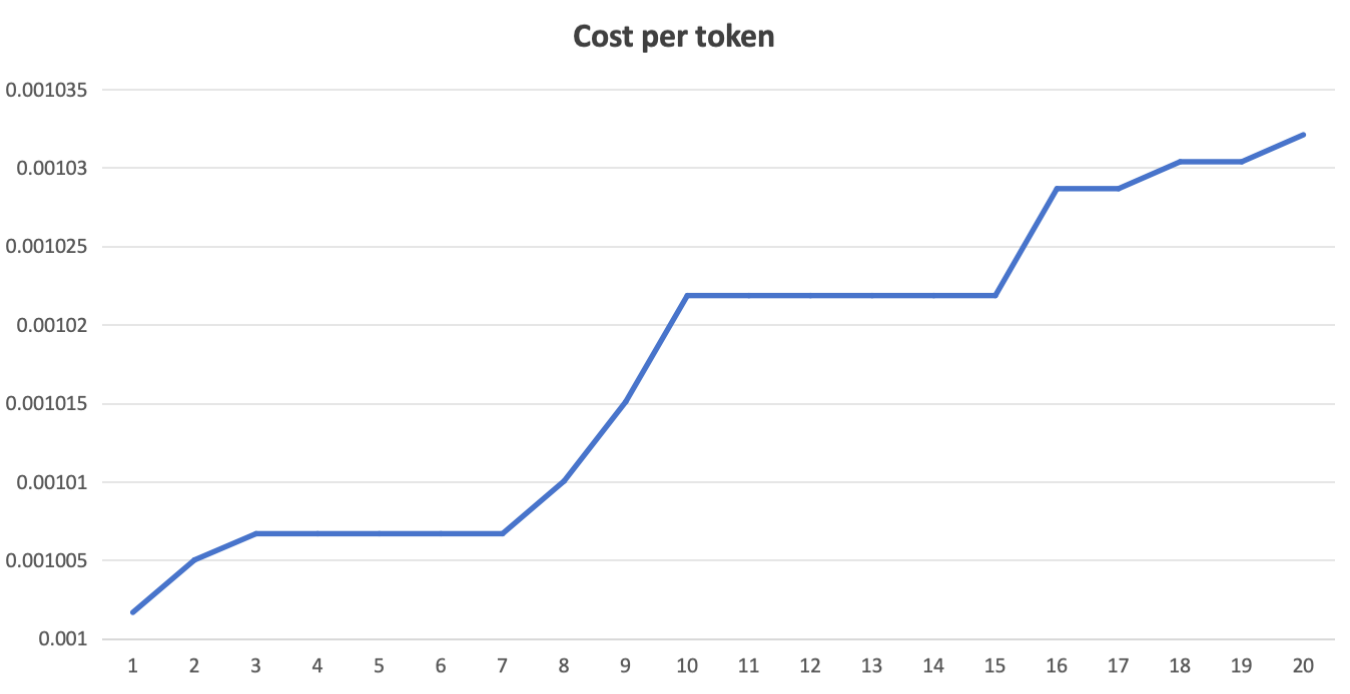
\includegraphics[width=400px]{image11}

\paragraph{2.3.1 -
按目标时间铸造}\label{ux6309ux76eeux6807ux65f6ux95f4ux94f8ux9020}

如果铸造速度过快,铸造成本将迅速增加。但如果按目标时间铸造,每个人将获得相同的代币成本。

以下是解释的表格:

\begin{longtable}[]{@{}
  >{\raggedright\arraybackslash}p{(\columnwidth - 10\tabcolsep) * \real{0.0603}}
  >{\raggedright\arraybackslash}p{(\columnwidth - 10\tabcolsep) * \real{0.1207}}
  >{\raggedright\arraybackslash}p{(\columnwidth - 10\tabcolsep) * \real{0.2845}}
  >{\raggedright\arraybackslash}p{(\columnwidth - 10\tabcolsep) * \real{0.1983}}
  >{\raggedright\arraybackslash}p{(\columnwidth - 10\tabcolsep) * \real{0.1983}}
  >{\raggedright\arraybackslash}p{(\columnwidth - 10\tabcolsep) * \real{0.1379}}@{}}
\toprule\noalign{}
\begin{minipage}[b]{\linewidth}\raggedright
周期
\end{minipage} & \begin{minipage}[b]{\linewidth}\raggedright
周期铸造时间
\end{minipage} & \begin{minipage}[b]{\linewidth}\raggedright
难度系数变化
\end{minipage} & \begin{minipage}[b]{\linewidth}\raggedright
难度系数
\end{minipage} & \begin{minipage}[b]{\linewidth}\raggedright
每次铸造规模
\end{minipage} & \begin{minipage}[b]{\linewidth}\raggedright
每代币成本
\end{minipage} \\
\midrule\noalign{}
\endhead
\bottomrule\noalign{}
\endlastfoot
1 & 589 & 0.000183333 & 1.000183333 & 99.98167003 & 0.001000183 \\
2 & 609 & 0 & 1.000183333 & 99.98167003 & 0.001000183 \\
3 & 596 & 6.66667E-05 & 1.000250012 & 99.97500503 & 0.00100025 \\
4 & 594 & 0.0001 & 1.000350037 & 99.96500853 & 0.00100035 \\
5 & 607 & 0 & 1.000350037 & 99.96500853 & 0.00100035 \\
6 & 609 & 0 & 1.000350037 & 99.96500853 & 0.00100035 \\
7 & 609 & 0 & 1.000350037 & 99.96500853 & 0.00100035 \\
8 & 608 & 0 & 1.000350037 & 99.96500853 & 0.00100035 \\
9 & 604 & 0 & 1.000350037 & 99.96500853 & 0.00100035 \\
10 & 608 & 0 & 1.000350037 & 99.96500853 & 0.00100035 \\
11 & 608 & 0 & 1.000350037 & 99.96500853 & 0.00100035 \\
12 & 607 & 0 & 1.000350037 & 99.96500853 & 0.00100035 \\
13 & 607 & 0 & 1.000350037 & 99.96500853 & 0.00100035 \\
14 & 605 & 0 & 1.000350037 & 99.96500853 & 0.00100035 \\
15 & 603 & 0 & 1.000350037 & 99.96500853 & 0.00100035 \\
16 & 589 & 0.000183333 & 1.000533435 & 99.94668497 & 0.001000533 \\
17 & 608 & 0 & 1.000533435 & 99.94668497 & 0.001000533 \\
18 & 590 & 0.000166667 & 1.00070019 & 99.93002996 & 0.0010007 \\
19 & 603 & 0 & 1.00070019 & 99.93002996 & 0.0010007 \\
20 & 611 & 0 & 1.00070019 & 99.93002996 & 0.0010007 \\
\end{longtable}

上述表格的代币成本图表如下:

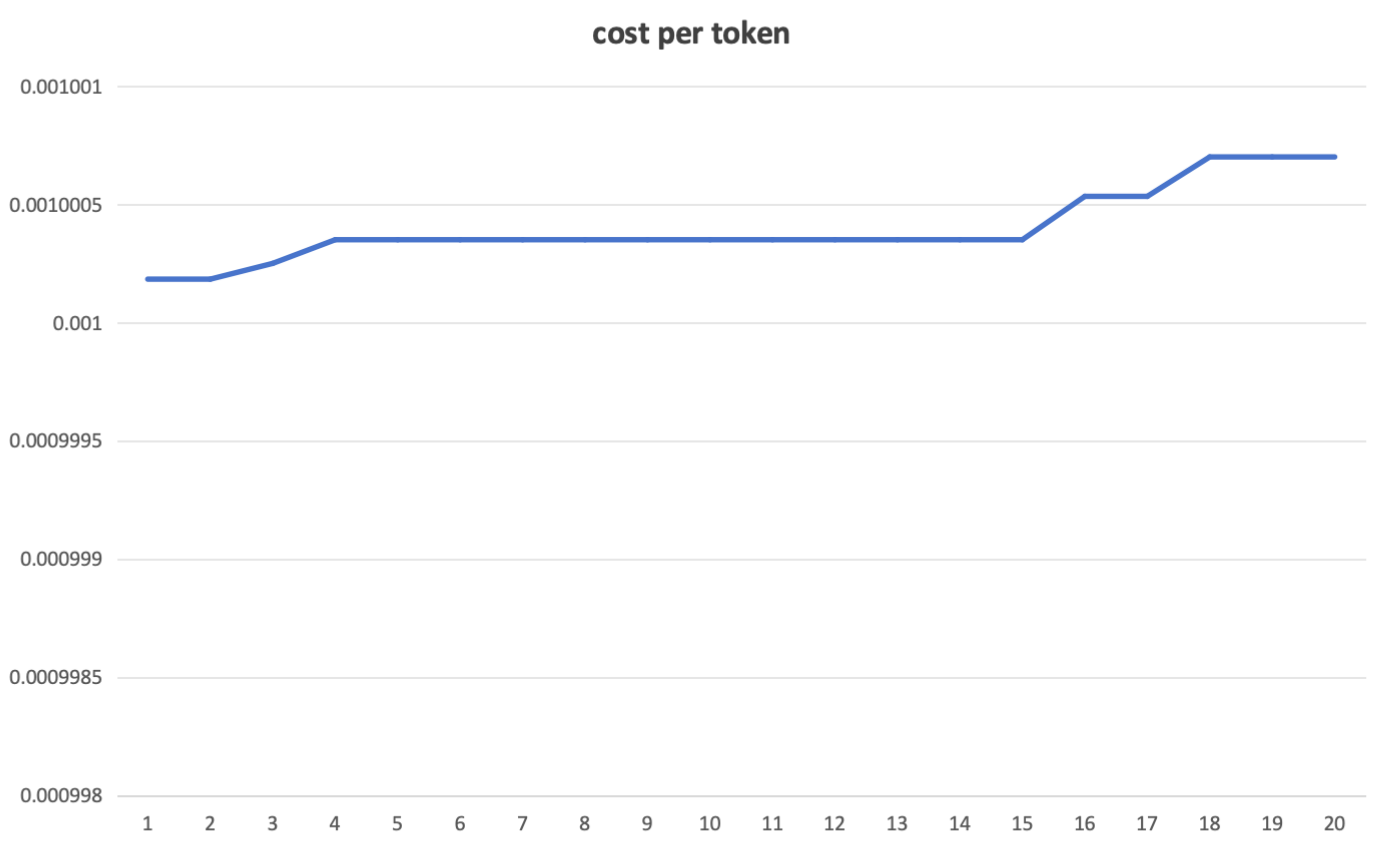
\includegraphics[width=400px]{image12}

\paragraph{2.3.2 -
关于周期基础铸造规模}\label{ux5173ux4e8eux5468ux671fux57faux7840ux94f8ux9020ux89c4ux6a21}

此外,\textbf{周期基础铸造规模}逐渐减少。假设\textbf{减少因子}为\textbf{3/4}:

\begin{itemize}
\item
  第一个\textbf{时代},\textbf{目标周期铸造规模}为\textbf{100,000代币},\textbf{周期基础铸造规模}为\textbf{100代币}。
\item
  第二个\textbf{时代},\textbf{目标周期铸造规模}为\textbf{100,000 * 3/4
  = 75,000代币},\textbf{周期基础铸造规模}为\textbf{75代币}。
\item
  第三个\textbf{时代},\textbf{目标周期铸造规模}为\textbf{75,000 * 3/4 =
  56,250代币},\textbf{周期基础铸造规模}为\textbf{56.25代币}。
\item
  \ldots{}
\end{itemize}

\subsubsection{2.4 - 优势}\label{ux4f18ux52bf}

\paragraph{2.4.1 - 优势1}\label{ux4f18ux52bf1}

如果\textbf{机器人}参与铸造,它们会发现铸造速度越快,获得的代币越少,成本越高。与许多试图阻止\textbf{机器人}参与铸造的方法相反,该提案不阻止机器人进行批量铸造。然而,高成本和低收益将阻止机器人。

\paragraph{2.4.2 - 优势2}\label{ux4f18ux52bf2}

如果\textbf{机器人}监控前一个\textbf{周期}的铸造时间以计算下一个\textbf{周期}的难度并评估是否参与,那么所有机器人必须拥有自己的策略。否则,趋同的策略将导致所有机器人蜂拥而至,造成收益大幅下降和成本大幅上升。因为机器人的收益不取决于铸造的``速度'',而更多取决于对其他机器人行为的``猜测'',大大增加了机器人的策略难度。

\paragraph{2.4.3 - 优势3}\label{ux4f18ux52bf3}

采用难度只增不减的机制,确保预期铸造成本始终上升。当难度迅速增加时,用户不会期待难度下降,要么继续铸造,要么停止铸造。这避免了等待难度下降导致的铸造停滞。

\paragraph{2.4.4 - 优势4}\label{ux4f18ux52bf4}

随着难度和铸造成本的增加,直到市场认为成本达到合理水平,铸造将放缓或停止。此时的铸造成本将成为代币市场价格的锚点。

\paragraph{2.4.5 - 优势5}\label{ux4f18ux52bf5}

从铸造中收集的资金用于去中心化交易所的流动性池。该提案避免了过去一些平台收取的固定铸造费用远不足以满足市场流动性需求的问题。随着难度增加,每次铸造的产出将减少,完成目标周期铸造规模所需的铸造次数将增加,从而提高铸造费用。增加的铸造费用将进入流动性池,为市场价值管理提供充足的流动性支持。

\paragraph{2.4.6 - 优势6}\label{ux4f18ux52bf6}

当市场价格下跌时,人们会发现铸造不再具有成本效益,导致铸造活动放缓或停止。低成本供应的增加将减少或停止,避免了价格下跌与代币供应持续增加的``死亡螺旋''陷阱。如果有新铸造者加入,难度和成本将再次上升。

\paragraph{2.4.7 - 优势7}\label{ux4f18ux52bf7}

铸造成本和难度完全取决于市场参与,没有中心化控制,在去中心化环境中实现动态平衡。

\begin{quote}
\mbox{}%
\paragraph{\texorpdfstring{\textbf{在最大利益原则的驱动下,最终铸造速度将趋向于目标设定,并实现纳什均衡}。}{在最大利益原则的驱动下,最终铸造速度将趋向于目标设定,并实现纳什均衡。}}\label{ux5728ux6700ux5927ux5229ux76caux539fux5219ux7684ux9a71ux52a8ux4e0bux6700ux7ec8ux94f8ux9020ux901fux5ea6ux5c06ux8d8bux5411ux4e8eux76eeux6807ux8bbeux5b9aux5e76ux5b9eux73b0ux7eb3ux4ec0ux5747ux8861}
\end{quote}

该机制有效激励早期参与者,对持续关注的社区成员非常友好,同时对投机者和通过技术手段作弊的人不友好。

\begin{quote}
我们在以太坊测试网\textbf{sepolia}(\textbf{solidity})和\textbf{Solana}(\textbf{rust/anchor})开发网上编码了\textbf{PoM}铸造算法,并将提供前端\textbf{Typescript}脚本供社区测试,同时开源\textbf{python}语言模拟代码。
\end{quote}

\subsection{3. 计算}\label{ux8ba1ux7b97}

\subsubsection{3.1 - 公式}\label{ux516cux5f0f}

\paragraph{3.1.1 -
当前周期的难度系数}\label{ux5f53ux524dux5468ux671fux7684ux96beux5ea6ux7cfbux6570}

\begin{itemize}
\tightlist
\item
  \(d\):难度系数
\item
  \(d'\):前一周期的难度系数
\item
  \(\delta d\):难度系数变化
\item
  \(N_e\):已过去周期的区块数
\item
  \(N_t\):每个周期的目标区块数
\end{itemize}

难度系数的变化基于实际时间与目标时间的比例计算。我们仅考虑已过去区块数低于每个周期目标区块数的情况。公式如下:

\begin{equation}
\delta d = \frac{1-\frac{N_e}{N_t}}{100},(N_e < N_t)
\end{equation} \begin{equation}
\delta d = 0,(N_e \geq N_t)
\end{equation}

\textbf{注意}:在上述公式中,100是用于控制难度增加比例在一定阈值范围内的因子。将其设置为100意味着难度增加的最大比例为1\%。如果将其设置为50,则难度增加的最大比例为2\%。

在得到难度系数变化后,当前周期的难度系数为:

\begin{equation}
d = d' * (1 + \delta d)
\end{equation}

对于可以准确获取区块时间戳的区块链,上述\textbf{区块数}可以替换为\textbf{时间戳}。

\textbf{示例:}

在2.3.1的示例中,每个\textbf{周期}的目标铸造时间为600秒。在\textbf{第十周期},铸造耗时200秒,\textbf{第九周期}的\textbf{难度系数}为\textbf{1.015086348},因此\textbf{第十周期}的新\textbf{难度系数}将调整为:
\textbf{1.015086348 * ((1 - 200 / 600) / 100 + 1) = 1.02185359}。

在\textbf{第十一周期},铸造耗时1000秒,超过目标铸造时间600秒,因此保持与\textbf{第十周期}相同的\textbf{难度系数},即\textbf{1.02185359}。

\paragraph{3.1.2 -
当前时代每次铸造的基础规模(Mb)}\label{ux5f53ux524dux65f6ux4ee3ux6bcfux6b21ux94f8ux9020ux7684ux57faux7840ux89c4ux6a21mb}

\begin{itemize}
\tightlist
\item
  \(M_b\):当前时代每次铸造的基础规模
\item
  \(M_0\):创世时代每次铸造的基础规模
\item
  \(f\):减少因子
\item
  \(e\):当前时代
\end{itemize}

\begin{equation}
M_b = M_0 * f^{e-1}
\end{equation}

\textbf{减少因子}

\begin{itemize}
\tightlist
\item
  \(f\)=0.5表示每个时代减少\textbf{50\%}(减半)
\item
  \(f\)=2/3表示每个时代减少\textbf{33.33\%}
\item
  \(f\)=3/4表示每个时代减少\textbf{25\%}
\item
  \(f\)=4/5表示每个时代减少\textbf{20\%}
\item
  \(f\)=5/6表示每个时代减少\textbf{1/6},等等。
\end{itemize}

\paragraph{3.1.3 -
当前时代每个周期的目标铸造规模}\label{ux5f53ux524dux65f6ux4ee3ux6bcfux4e2aux5468ux671fux7684ux76eeux6807ux94f8ux9020ux89c4ux6a21}

\begin{itemize}
\tightlist
\item
  \(T\):当前时代每个周期的目标铸造规模
\item
  \(T_0\):创世时代每个周期的目标铸造规模
\item
  \(f\):减少因子
\item
  \(e\):当前时代
\end{itemize}

\begin{equation}
 T = T_0 * f^{e-1}
\end{equation}

\paragraph{3.1.4 -
当前周期每次铸造的规模}\label{ux5f53ux524dux5468ux671fux6bcfux6b21ux94f8ux9020ux7684ux89c4ux6a21}

\begin{itemize}
\tightlist
\item
  \(M\):当前周期每次铸造的规模
\item
  \(M_b\):当前时代每次铸造的基础规模
\item
  \(d\):难度系数
\end{itemize}

\begin{equation}
M = \frac{M_b}{d}
\end{equation}

\textbf{示例:}

在2.3.1的示例中,当前时代的\textbf{每次铸造的基础规模}为\textbf{100代币},\textbf{第十六周期}的\textbf{难度系数}为\textbf{1.028665947},那么铸造规模为:\textbf{100
/ 1.028665947 = 97.213289代币}。

\paragraph{3.1.5}\label{section}

如果\(T\)不是\(M\)的整数倍,需要对\(M\)进行调整,即:

\begin{equation}
M_a = \frac{T}{\lfloor\frac{T}{M}\rfloor + 1}, (T \nmid M)
\end{equation}

如果\(T\)是\(M\)的整数倍,则无需如上调整。 \begin{equation}
M_a = M, (T \mid M)
\end{equation}

\paragraph{3.1.6 - 代币成本}\label{ux4ee3ux5e01ux6210ux672c}

尽管每次铸造的费用保持不变,但随着难度增加,每次铸造获得的代币数量将减少,因此代币成本将增加。

以下是计算代币成本的方法。

\begin{itemize}
\tightlist
\item
  \(P_0\):铸造费用
\item
  \(p\):代币成本
\end{itemize}

\begin{equation}
p = \frac{P_0}{M_a}
\end{equation} 如果\textbf{T}不是\textbf{M}的整数倍,价格为:
\begin{equation}
p = \frac{P_0*(\lfloor\frac{T_0}{M_0}*d\rfloor + 1)}{T_0*f^{e-1}}, (T \nmid M)
\end{equation} \begin{equation}
p = \frac{P_0}{M_0*f^{e-1}}*d, (T \mid M)
\end{equation}
由于\(P_0\)、\(T_0\)、\(M_0\)、\(f\)和\(e\)在一个时代内是常数,我们知道:\(p \propto d\)。

\paragraph{3.1.7}\label{section-1}

\(T\)和\(M\)随着每个\textbf{时代}呈指数减少,但两者之间的比例保持不变,无论在哪个\textbf{时代}。

\begin{equation}
T=T_0*f^{e-1}
\end{equation} \begin{equation}
M = \frac{M_b}{d}=\frac{M_0 * f^{e-1}}{d}
\end{equation} \begin{equation}
\frac{T}{M} = \frac{T_0}{M_0} * d
\end{equation}

\paragraph{3.1.8}\label{section-2}

如果\(N_t\)设为10分钟,那么理论上每次铸造的目标间隔时间为:600秒 / 33 =
18.18秒每次。

如果间隔时间较长,意味着完成一个\textbf{周期}的所有铸造需要比计划时间(10分钟)更长,这意味着铸造者较少,在这种情况下,难度降低,每次铸造的奖励增加。

反之,如果间隔时间较短,表明完成一个\textbf{周期}的铸造时间少于计划时间(10分钟),这意味着铸造者较多,在这种情况下,难度增加,每次铸造的奖励减少。

\subsubsection{3.2 -
计算周期铸造规模的关键代码(Rust)}\label{ux8ba1ux7b97ux5468ux671fux94f8ux9020ux89c4ux6a21ux7684ux5173ux952eux4ee3ux7801rust}

\begin{Shaded}
\begin{Highlighting}[numbers=left,,]
\KeywordTok{pub} \KeywordTok{fn}\NormalTok{ get\_mint\_size(}
\NormalTok{  config\_data}\OperatorTok{:} \OperatorTok{\&}\NormalTok{TokenConfigData}\OperatorTok{,}
\NormalTok{) }\OperatorTok{{-}\textgreater{}} \DataTypeTok{Result}\OperatorTok{\textless{}}\NormalTok{(}\DataTypeTok{u64}\OperatorTok{,} \DataTypeTok{f64}\OperatorTok{,} \DataTypeTok{u64}\NormalTok{)}\OperatorTok{\textgreater{}} \OperatorTok{\{}
  \KeywordTok{let}\NormalTok{ delta\_difficulty\_coefficient }\OperatorTok{=} \ControlFlowTok{if}\NormalTok{ config\_data}\OperatorTok{.}\NormalTok{mint\_state\_data}\OperatorTok{.}\NormalTok{elapsed\_seconds\_epoch}
    \OperatorTok{\textless{}}\NormalTok{ config\_data}\OperatorTok{.}\NormalTok{target\_seconds\_per\_epoch }\OperatorTok{\{}
\NormalTok{    (}\DecValTok{1.0} \OperatorTok{{-}}\NormalTok{ config\_data}\OperatorTok{.}\NormalTok{mint\_state\_data}\OperatorTok{.}\NormalTok{elapsed\_seconds\_epoch}\OperatorTok{.}\NormalTok{safe\_as\_f64()}\OperatorTok{?} \OperatorTok{/} 
\NormalTok{       config\_data}\OperatorTok{.}\NormalTok{target\_seconds\_per\_epoch}\OperatorTok{.}\NormalTok{safe\_as\_f64()}\OperatorTok{?}\NormalTok{) }\OperatorTok{/} \DecValTok{100.0}
  \OperatorTok{\}} \ControlFlowTok{else} \OperatorTok{\{}
    \DecValTok{0.0}
  \OperatorTok{\};}
  \KeywordTok{let}\NormalTok{ difficulty\_coefficient }\OperatorTok{=}\NormalTok{ config\_data}\OperatorTok{.}\NormalTok{mint\_state\_data}\OperatorTok{.}\NormalTok{difficulty\_coefficient\_epoch }
    \OperatorTok{*}\NormalTok{ (}\DecValTok{1.0} \OperatorTok{+}\NormalTok{ delta\_difficulty\_coefficient)}\OperatorTok{;}
  \KeywordTok{let}\NormalTok{ base\_mint\_size }\OperatorTok{=}\NormalTok{ config\_data}\OperatorTok{.}\NormalTok{initial\_mint\_size}\OperatorTok{.}\NormalTok{safe\_as\_f64()}\OperatorTok{?} 
    \OperatorTok{*}\NormalTok{ config\_data}\OperatorTok{.}\NormalTok{reduce\_ratio}\OperatorTok{.}\NormalTok{powf((config\_data}\OperatorTok{.}\NormalTok{mint\_state\_data}\OperatorTok{.}\NormalTok{current\_era }\OperatorTok{{-}} \DecValTok{1}\NormalTok{)}\OperatorTok{.}\NormalTok{safe\_as\_f64()}\OperatorTok{?}\NormalTok{)}\OperatorTok{;}
  \KeywordTok{let}\NormalTok{ base\_target\_mint\_size\_per\_epoch }\OperatorTok{=}\NormalTok{ config\_data}\OperatorTok{.}\NormalTok{initial\_target\_mint\_size\_per\_epoch}\OperatorTok{.}\NormalTok{safe\_as\_f64()}\OperatorTok{?} 
    \OperatorTok{*}\NormalTok{ config\_data}\OperatorTok{.}\NormalTok{reduce\_ratio}\OperatorTok{.}\NormalTok{powf((config\_data}\OperatorTok{.}\NormalTok{mint\_state\_data}\OperatorTok{.}\NormalTok{current\_era }\OperatorTok{{-}} \DecValTok{1}\NormalTok{)}\OperatorTok{.}\NormalTok{safe\_as\_f64()}\OperatorTok{?}\NormalTok{)}\OperatorTok{;}
  \KeywordTok{let}\NormalTok{ mint\_size }\OperatorTok{=}\NormalTok{  base\_mint\_size }\OperatorTok{/}\NormalTok{ difficulty\_coefficient}\OperatorTok{;}
  \KeywordTok{let}\NormalTok{ target\_mint\_size\_epoch }\OperatorTok{=}\NormalTok{ (base\_target\_mint\_size\_per\_epoch }\OperatorTok{/}\NormalTok{ mint\_size)}\OperatorTok{.}\NormalTok{trunc() }
  \OperatorTok{*}\NormalTok{ mint\_size}\OperatorTok{;}
  \ConstantTok{Ok}\NormalTok{((mint\_size}\OperatorTok{.}\NormalTok{safe\_as\_u64()}\OperatorTok{?,}\NormalTok{ difficulty\_coefficient}\OperatorTok{,}\NormalTok{ target\_mint\_size\_epoch}\OperatorTok{.}\NormalTok{safe\_as\_u64()}\OperatorTok{?}\NormalTok{))}
\OperatorTok{\}}
\end{Highlighting}
\end{Shaded}

\subsection{4. 部署参数}\label{ux90e8ux7f72ux53c2ux6570}

\subsubsection{4.1 总供应量}\label{ux603bux4f9bux5e94ux91cf}

与普通代币发行模式不同,\textbf{PoM}的\textbf{总供应量}基于\textbf{时代}、\textbf{周期}和\textbf{减少因子}计算。

确定总供应量的四个参数:

\begin{itemize}
\tightlist
\item
  \(E\):总时代数
\item
  \(C\):每个时代的周期数
\item
  \(T_0\):初始周期目标铸造规模
\item
  \(f\):时代减少因子,\(f \in (0,1)\)
\end{itemize}

\textbf{计算}

\begin{equation}
TotalSupply = \sum_{i=1}^{E}(C \cdot T_0 \cdot f^{i-1})=C \cdot T_0 \cdot \frac{1-f^E}{1-f}
\end{equation}

\textbf{示例:}

\(E\)=15, \(C\)=10, \(T_0\)=100,000代币, \(f\)=0.75

\textbf{总供应量为:} 3,946,546.156代币

\href{https://www.wolframalpha.com/input?i=sum+10*100000*0.75\%5E\%28i-1\%29\%2C+i+\%3D+1+to+15}{点击此处打开Wolfram计算},您可以使用\textbf{Wolfram}轻松计算总供应量。

\paragraph{4.1.1 -
最大总供应量}\label{ux6700ux5927ux603bux4f9bux5e94ux91cf}

当\(E\)趋向无穷大,意味着铸造可以无限期进行,\textbf{总供应量}将收敛到一个值,即:

\textbf{计算}

\begin{equation}
lim_{E→\infty}(\cdot C \cdot T_0\cdot\frac{1-f^E}{1-f})=C \cdot T_0\cdot \frac{1-f^{\infty}}{1-f}=\frac{C\cdot T_0}{1-f}
\end{equation}

\textbf{示例:}

\(C\)=10, \(T_0\)=100,000代币, \(f\)=0.75

\textbf{总供应量为:} 4,000,000代币

\subsubsection{4.2
预计总铸造时间:}\label{ux9884ux8ba1ux603bux94f8ux9020ux65f6ux95f4}

\textbf{注意:} 实际总铸造时间将与预计总铸造时间不同。

以下是计算预计总铸造时间的公式。

\begin{itemize}
\tightlist
\item
  \(E\):时代
\item
  \(C\):每个时代的周期数
\item
  \(N_t\):每个周期的目标区块数
\item
  \(t\):每个区块的秒数
\end{itemize}

\textbf{计算}

\begin{equation}
TotalEstimatedTime = E \cdot C \cdot N_t \cdot t
\end{equation}

\textbf{示例:} \(E\)=15, \(C\)=10, \(N_t\)=50, \(t\)=12秒

\textbf{预计总铸造时间:} 15 * 10 * 50 * 12 = 90,000秒 = 25小时

\subsubsection{4.3 总时代数}\label{ux603bux65f6ux4ee3ux6570}

结合上述两个公式,我们可以计算当铸造了80\%总供应量(\(r\))时的总时代数\(E_r\)。

\begin{equation}
C \cdot T_0 \cdot \frac{1-f^{E_r}}{1-f} = \frac{C \cdot T_0}{1-f}*r
\end{equation} 从该方程中,我们得到: \begin{equation}
E_r = \log_f(1-r)
\end{equation}

\textbf{示例:}

\(r\)=80\%, \(f\)=0.75, 则
\(E_r\)=\(\log_{0.75}(1-0.8)=\frac{\ln0.2}{\ln0.75}=5.59\)。

这意味着在第六个时代中期,80\%的总供应量将被铸造。

如果\(C=10\),在第56个周期(5.59*10),80\%的总供应量将被铸造。

\subsubsection{4.4 总铸造费用}\label{ux603bux94f8ux9020ux8d39ux7528}

每次铸造需要支付固定费用,然而,由于难度的增加,同一周期内的铸造次数将增加,每次铸造获得的代币数量将减少,因此总费用将相应增加。

\begin{quote}
\textbf{注意:} 这些铸造费用将自动添加到流动性池中。
\end{quote}

\begin{itemize}
\tightlist
\item
  \(Fee\):总费用
\item
  \(P_0\):每次铸造的费用
\item
  \(d\):难度系数
\item
  \(Q\):一个周期内的铸造次数
\item
  \(T_0\):创世时代每个周期的目标铸造规模
\item
  \(M_0\):创世时代每次铸造的基础规模
\item
  \(C_e\):已过去的周期数,\(C_e = E * C\)
\end{itemize}

一个周期内的铸造次数:

\begin{equation}
Q = {\lfloor{\frac{T_0}{M_0}*d}\rfloor + 1}, (T_0 \nmid M_0)
\end{equation}

\begin{equation}
Q = \frac{T_0}{M_0}*d, (T_0 \mid M_0)
\end{equation} 为简化起见,假设\(T_0 \mid M_0\),总费用为:

\begin{equation}
TotalFee = \sum_{i=1}^{C_e}(P_0 \cdot Q_i)=\sum_{i=1}^{C_e}(\frac{P_0 \cdot T_0}{M_0}*d_i)
\end{equation}

由于\(d_i = d_{i-1} \cdot (1 + \delta d_i)\),
\(\delta d \in [0,0.01]\)(见3.1.1),且\(d_0=1\),总费用范围为:

\begin{equation}
TotalFee \in [\frac{P_0 \cdot T_0}{M_0} \cdot \sum_{i=1}^{C_e}1^i, \frac{P_0 \cdot T_0}{M_0} \cdot 101 \cdot (1.01^{C_e}-1)]
\end{equation}

简化后:

\begin{equation}
TotalFee \in [\frac{P_0 \cdot T_0}{M_0} \cdot C_e, \frac{P_0 \cdot T_0}{M_0} \cdot 101 \cdot (1.01^{C_e}-1)]
\end{equation}

\textbf{示例}

\(P_0=1\)美元, \(T_0=9000\), \(M_0=100\), \(d=1.5\),
\(C_e=300\),最低总费用为27,000美元,最高为169,096.2美元。

这表明,如果铸造速度很快,周期内的实际铸造时间(\(N_e\))少于目标时间(\(N_t\)),将导致难度和铸造成本持续增加。因此,收集的总费用将比难度保持不变时高出\textbf{6.3}倍,且随着周期数增加,差异将更加显著。

\subsubsection{4.5 使用案例}\label{ux4f7fux7528ux6848ux4f8b}

\paragraph{4.5.1}\label{section-3}

如果目标总供应量为2100万(左右),可以有(但不限于)以下参数组合:

\begin{longtable}[]{@{}
  >{\raggedright\arraybackslash}p{(\columnwidth - 22\tabcolsep) * \real{0.0833}}
  >{\raggedright\arraybackslash}p{(\columnwidth - 22\tabcolsep) * \real{0.0833}}
  >{\raggedright\arraybackslash}p{(\columnwidth - 22\tabcolsep) * \real{0.0833}}
  >{\raggedright\arraybackslash}p{(\columnwidth - 22\tabcolsep) * \real{0.0833}}
  >{\raggedright\arraybackslash}p{(\columnwidth - 22\tabcolsep) * \real{0.0833}}
  >{\raggedright\arraybackslash}p{(\columnwidth - 22\tabcolsep) * \real{0.0833}}
  >{\raggedright\arraybackslash}p{(\columnwidth - 22\tabcolsep) * \real{0.0833}}
  >{\raggedright\arraybackslash}p{(\columnwidth - 22\tabcolsep) * \real{0.0833}}
  >{\raggedright\arraybackslash}p{(\columnwidth - 22\tabcolsep) * \real{0.0833}}
  >{\raggedright\arraybackslash}p{(\columnwidth - 22\tabcolsep) * \real{0.0833}}
  >{\raggedright\arraybackslash}p{(\columnwidth - 22\tabcolsep) * \real{0.0833}}
  >{\raggedright\arraybackslash}p{(\columnwidth - 22\tabcolsep) * \real{0.0833}}@{}}
\toprule\noalign{}
\begin{minipage}[b]{\linewidth}\raggedright
\(C\)
\end{minipage} & \begin{minipage}[b]{\linewidth}\raggedright
\(T_0\)
\end{minipage} & \begin{minipage}[b]{\linewidth}\raggedright
\(M_0\)
\end{minipage} & \begin{minipage}[b]{\linewidth}\raggedright
\(f\)
\end{minipage} & \begin{minipage}[b]{\linewidth}\raggedright
\(N_t\)
\end{minipage} & \begin{minipage}[b]{\linewidth}\raggedright
\(t\)
\end{minipage} & \begin{minipage}[b]{\linewidth}\raggedright
总供应量
\end{minipage} & \begin{minipage}[b]{\linewidth}\raggedright
时代
\end{minipage} & \begin{minipage}[b]{\linewidth}\raggedright
周期
\end{minipage} & \begin{minipage}[b]{\linewidth}\raggedright
天数
\end{minipage} & \begin{minipage}[b]{\linewidth}\raggedright
最低总费用
\end{minipage} & \begin{minipage}[b]{\linewidth}\raggedright
最高总费用
\end{minipage} \\
\midrule\noalign{}
\endhead
\bottomrule\noalign{}
\endlastfoot
600 & 9000 & 1000 & 0.75 & 2000 & 12 & 2160万 & 10.413 & 6248 & 1735.56
& 56,241 & 9.088e29 \\
500 & 11000 & 1000 & 0.75 & 500 & 12 & 2200万 & 10.413 & 5206 & 361.57 &
57,277 & 3.49e25 \\
2500 & 1000 & 100 & 0.75 & 1000 & 0.4 & 1000万 & 10.413 & 26032 & 120.5
& 260,320 & 3.15e115 \\
\end{longtable}

\textbf{注意:}

\begin{itemize}
\item
  \(Eras = \log_f(1-0.95)\),铸造率为95\%
\item
  \(Epoches = Eras * C\)
\item
  \(days = Epoches * N_t * t / 3600 / 24\) =
  \(log_f(1-0.95) * C * N_t * t / 86400\)
\item
  由于\(f\)、\(t\)是固定的,总天数取决于\(C\)和\(N_t\)
\end{itemize}

\paragraph{4.5.2
如何计算所有参数}\label{ux5982ux4f55ux8ba1ux7b97ux6240ux6709ux53c2ux6570}

我们将根据以下条件尝试计算所有参数:

\begin{itemize}
\tightlist
\item
  总供应量
\item
  目标铸造天数
\item
  最低总费用
\end{itemize}

常量为:

\begin{itemize}
\tightlist
\item
  总供应量:10,000,000
\item
  目标铸造天数:180天,95\%的总供应量将被铸造
\item
  目标铸造费用:30,000美元
\item
  \(f\) = 0.75
\item
  \(T_0\) = 10,000
\item
  \(M_0\) = 1,000
\item
  \(t\)=0.4秒(用于Solana区块链)
\end{itemize}

\textbf{计算}

1-
\(\because TotalSupply = C \cdot T_0 / (1-f)\),所以每个时代的初始周期数(C)为:

\(C = TotalSupply \cdot (1 - f) / T_0\) = 10,000,000*(1-0.75)/10000=250

2- 根据以下公式,我们可以得到\(N_t = 14935\) \begin{equation}
C * N_t * t * \log_f(1-0.95) = 180天 * 86400秒/天
\end{equation}

3- 根据以下公式,我们可以得到\(C_e = 2603\) \begin{equation}
C_e = Eras * C = \log_f(1-0.95) * C = 10.413 * 250 = 2603
\end{equation}

4-
我们已经知道:\(T_0=10,000\),\(C_e=2603\),\(M_0=1000\),最低总费用公式:

\begin{equation}
\frac{P_0 * T_0 * (C_e+1)}{M_0} = P_0 * 10,000 * 2604 / 1000 = 300,000
\end{equation}

根据最低总费用公式,我们可以得到\(P_0 = 11.52\)美元,这意味着每个代币的最低价格为
\(P_0 / M_0 = 11.52 / 1000 = 0.01152\)美元

\href{https://docs.google.com/spreadsheets/d/1z4eO1k14noxTMcgADMc-I0xFXT0giMFPSBEGal4suvI/edit?usp=sharing}{点击此处打开在线计算器}

\subsection{5. 测试与评估}\label{ux6d4bux8bd5ux4e0eux8bc4ux4f30}

以下是模拟测试的参数:

\begin{itemize}
\tightlist
\item
  铸造间隔时间范围:0-30秒随机
\item
  总时代数:10
\item
  每个时代的周期数:20
\item
  最低难度系数:0.2
\item
  减少系数:3/4
\item
  创世时代每次铸造的基础规模:50
\item
  创世时代每个周期的目标铸造规模:200
\end{itemize}

\subsubsection{铸造奖励}\label{ux94f8ux9020ux5956ux52b1}

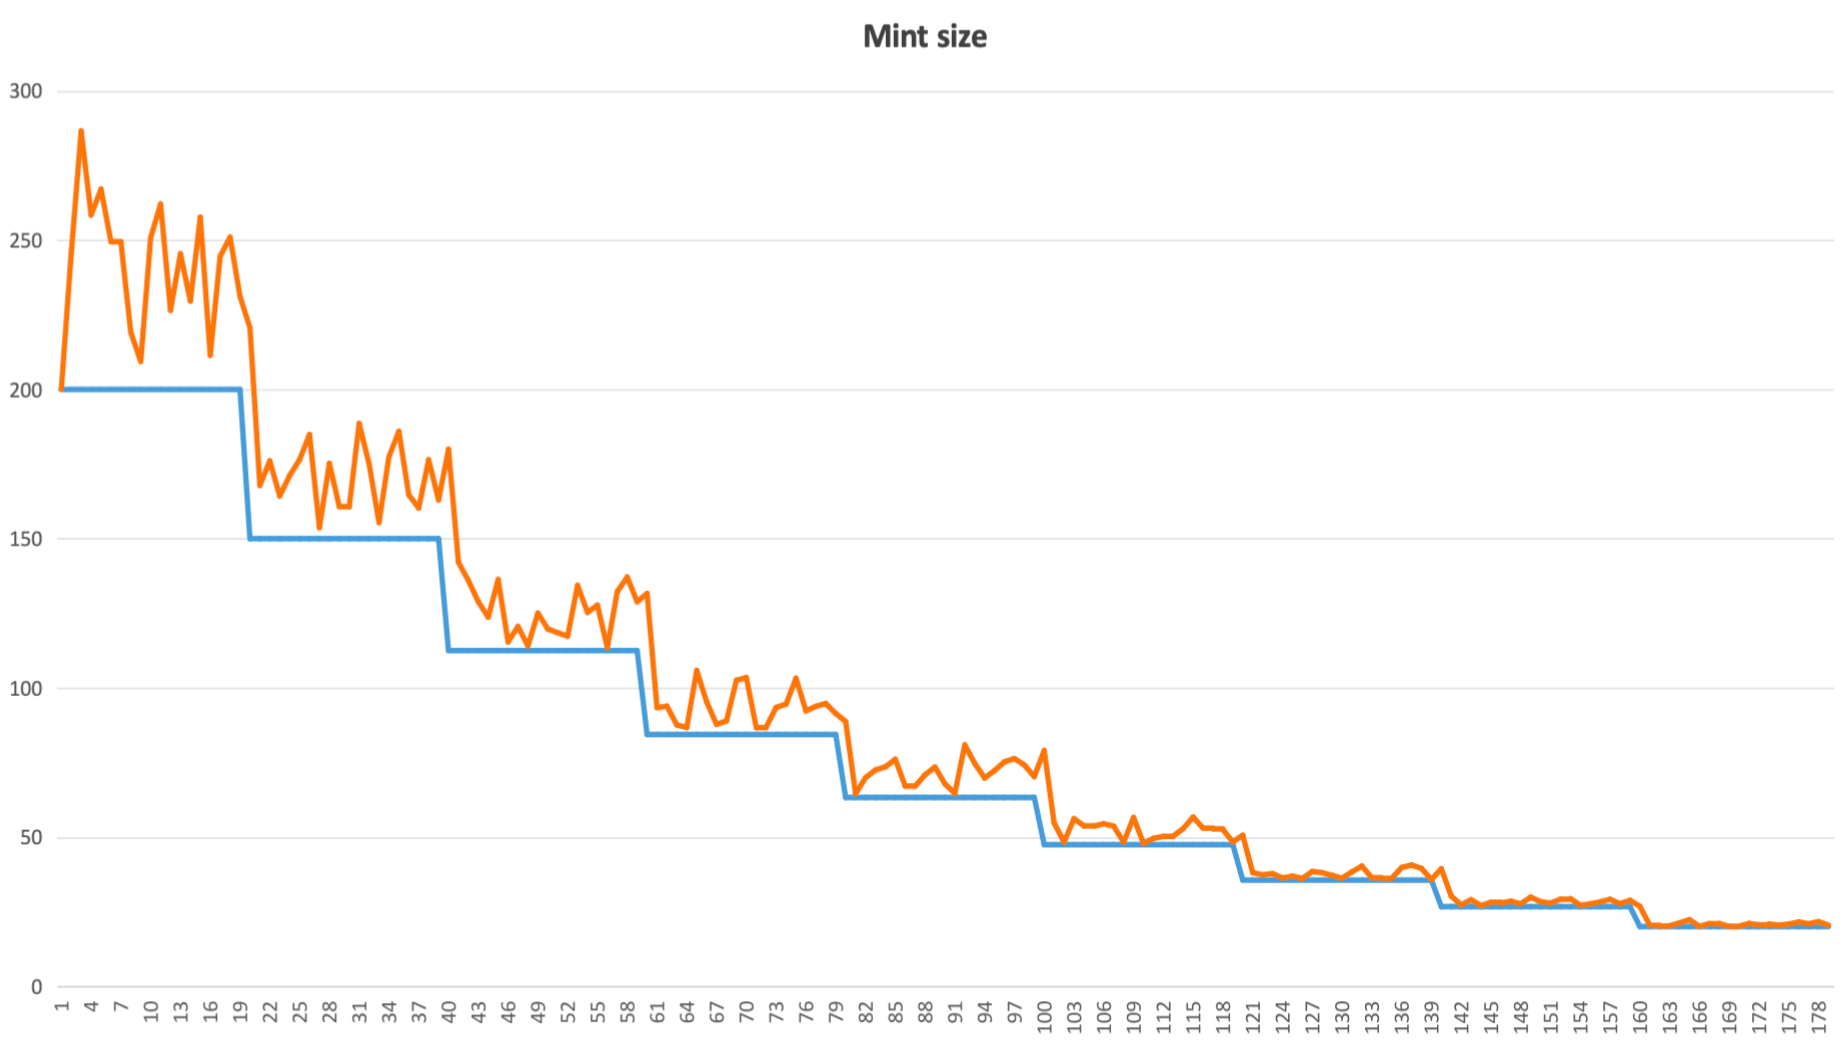
\includegraphics[width=400px]{image}

周期实际铸造收益与目标铸造收益对比

橙色线条表示\textbf{当前周期的实际铸造规模},蓝色线条表示\textbf{每次铸造的目标铸造规模},显示每个时代减少25\%的趋势。

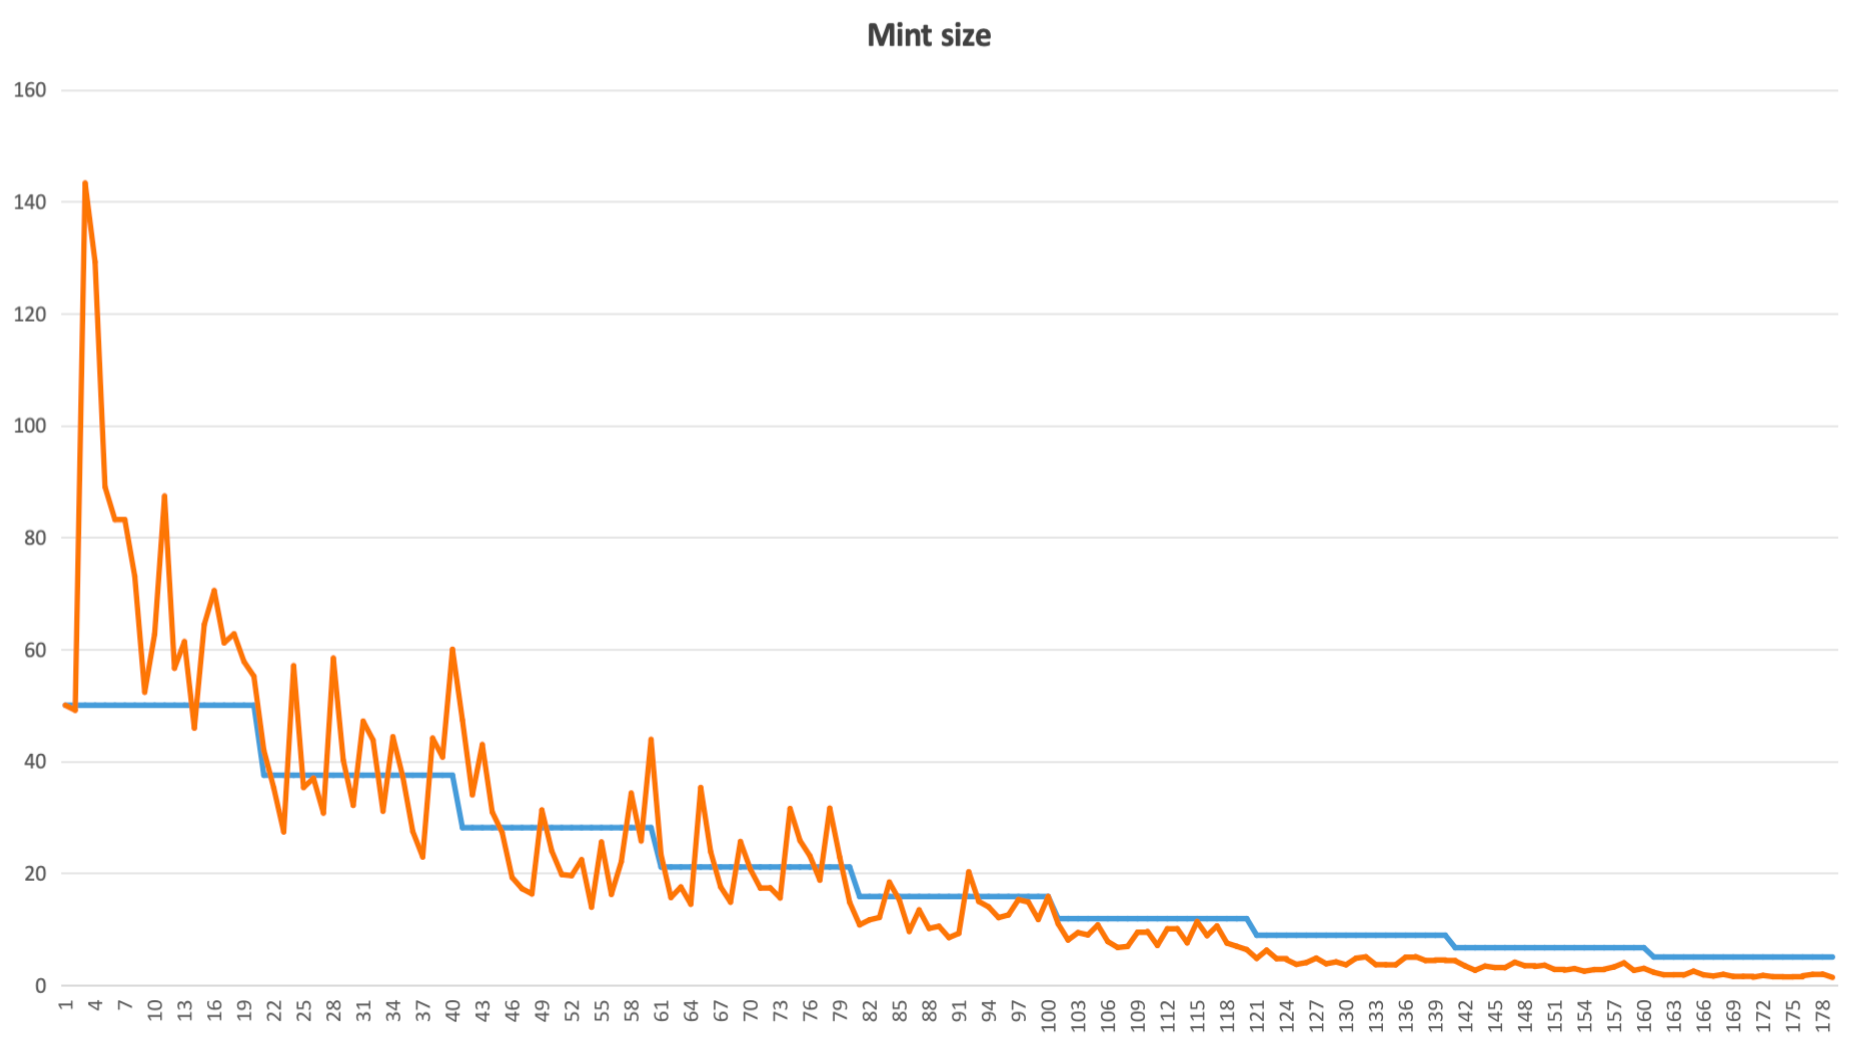
\includegraphics[width=400px]{image1}

实际铸造奖励与目标铸造奖励

橙色线条表示\textbf{实际铸造规模},蓝色线条表示\textbf{目标铸造规模}。

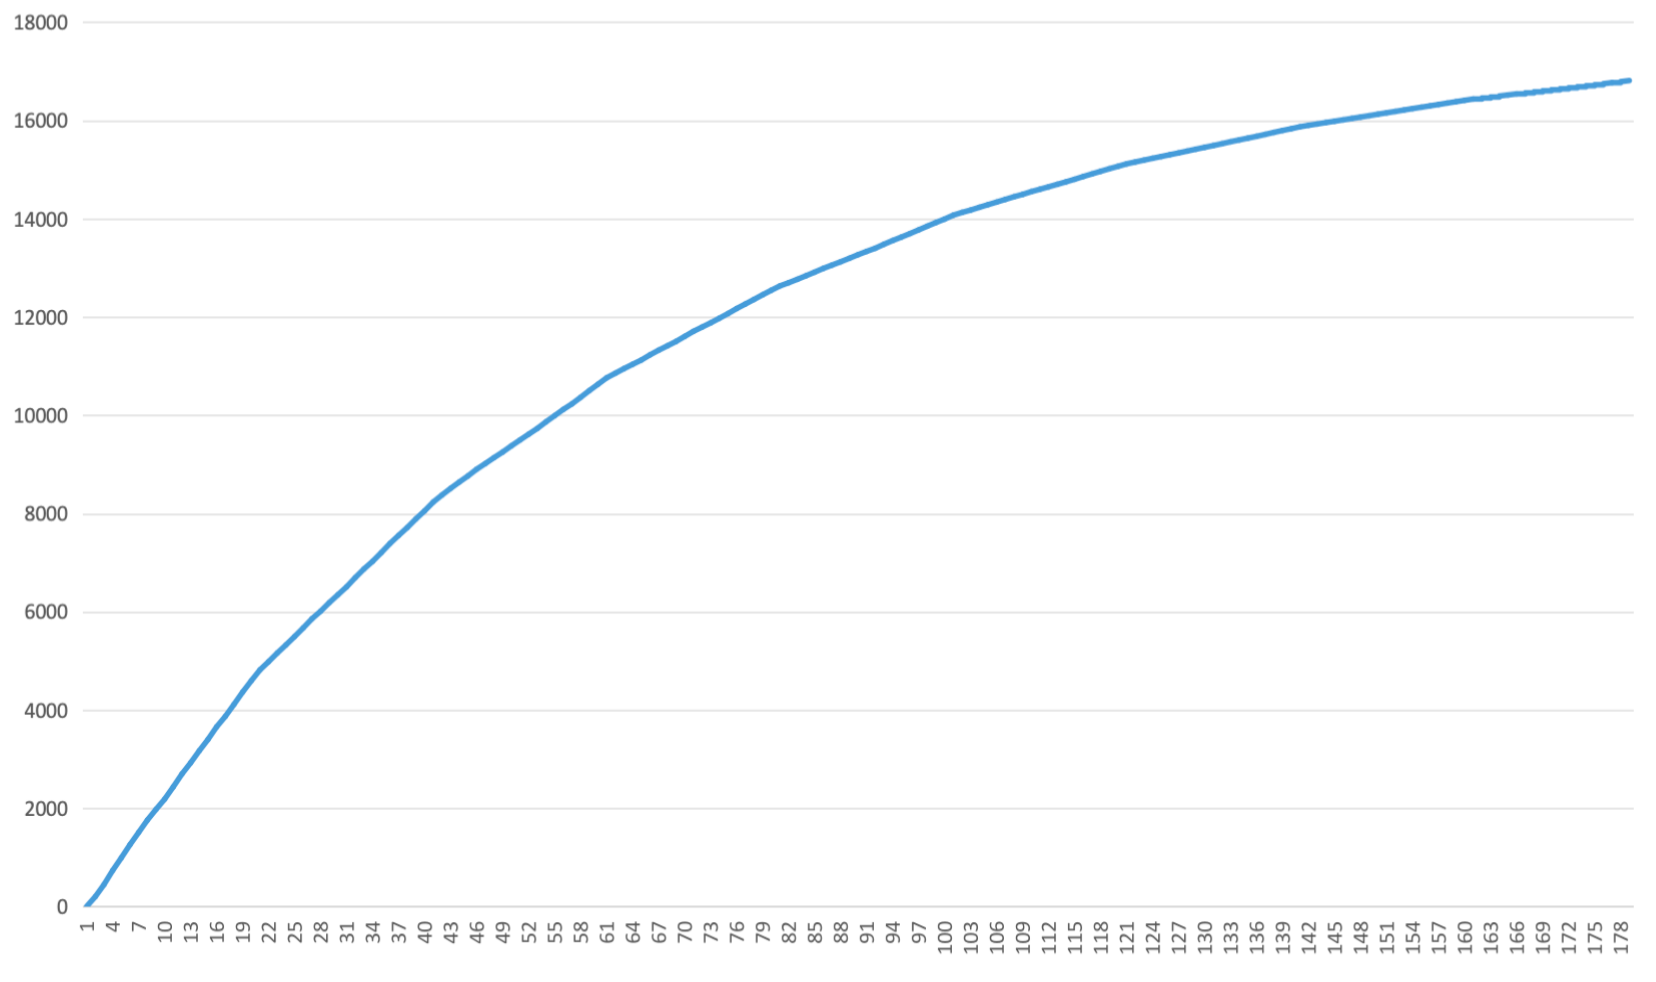
\includegraphics[width=400px]{image2}

总铸造曲线

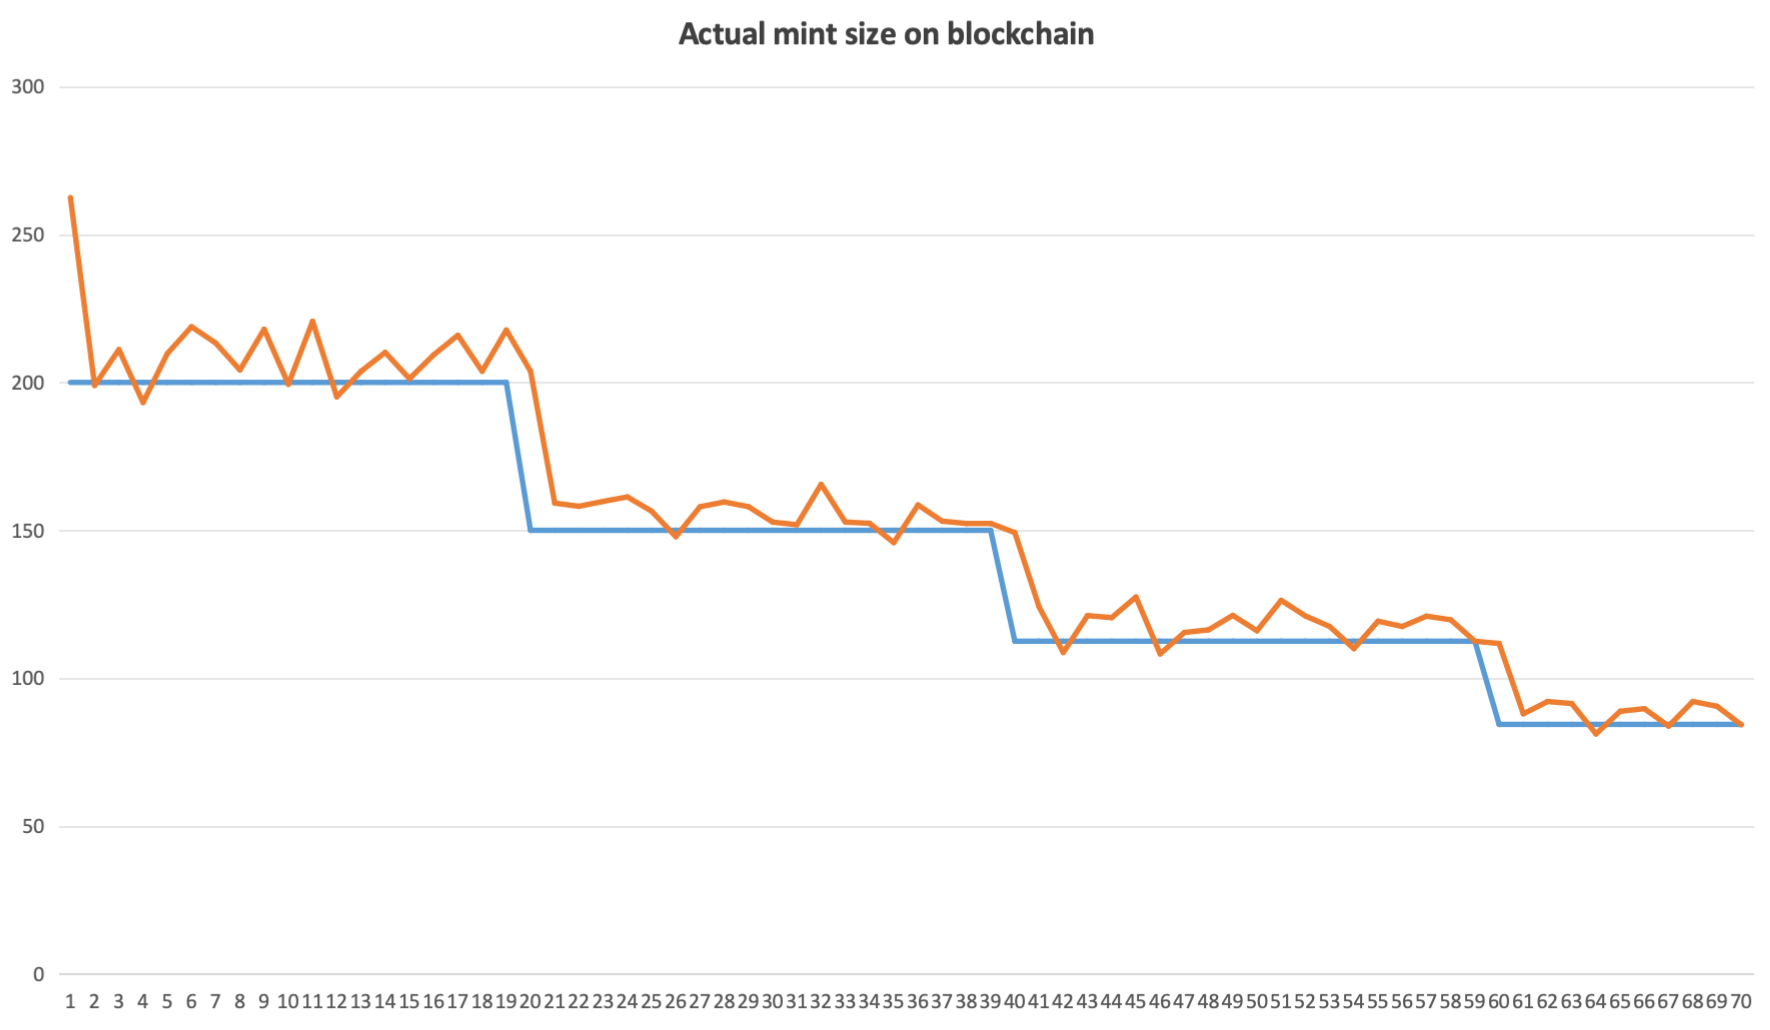
\includegraphics[width=400px]{image3}

以太坊链上的模拟结果

以上是在以太坊链上的模拟结果。

\subsection{6. 联盟铸造计划}\label{ux8054ux76dfux94f8ux9020ux8ba1ux5212}

\subsubsection{6.1 - 描述}\label{ux63cfux8ff0}

\textbf{联盟铸造计划}(\textbf{AMP})允许每个用户生成一个\textbf{唯一推荐码}(\textbf{URC})并与他人分享。当他人使用此\textbf{URC}进行铸造时,他们可以获得铸造费用的折扣,推荐者可以获得一些奖励。\textbf{AMP}设计为去中心化和社区驱动,激励建立更好的社区。

\begin{enumerate}
\def\labelenumi{\arabic{enumi}.}
\tightlist
\item
  去中心化与社区驱动

  \begin{itemize}
  \tightlist
  \item
    所有铸造必须使用\textbf{URC},每次铸造都与社区中的某个成员相关联。
  \item
    铸造的进度和速度受社区成员分享\textbf{URC}的影响,而不是由核心团队或某些大户控制。
  \item
    通过\textbf{AMP},社区更容易形成共识并吸引更多成员参与社区。
  \end{itemize}
\item
  激励社区

  \begin{itemize}
  \tightlist
  \item
    双重激励:推荐者(代码分享者)和使用\textbf{URC}的铸造者都能受益,这种双重激励机制有助于社区的增长和活跃度。
  \end{itemize}
\item
  铸造折扣与推荐者奖励

  \begin{itemize}
  \tightlist
  \item
    铸造费用折扣与提供\textbf{URC}的账户的代币余额挂钩。推荐者的余额越多,铸造折扣越高,铸造费用越低。这将鼓励参与者持有更多代币而不是全部出售。
  \item
    \textbf{URC}分享者可以获得稳定的奖励,这些奖励在铸造发生时由链上货币(以太坊的ETH或Solana的SOL)自动分配到推荐者的账户。
  \end{itemize}
\item
  铸造费用与难度调整

  \begin{itemize}
  \tightlist
  \item
    动态难度:铸造的总成本和难度将根据社区动态调整;铸造人数越多,铸造速度越快,总铸造成本越高,额外铸造费用也越高。
  \item
    部分铸造费用作为折扣重新分配给铸造者,作为奖励分配给\textbf{URC}分享者。
  \end{itemize}
\end{enumerate}

\begin{equation}
ExtraMintFee = \frac{P_0 \cdot T_0}{M_0} \cdot (\sum_{i=0}^{C_e}d_i - C_e - 1)
\end{equation} 该公式表明,\(d_i\)越高(大致高于1),额外铸造费用越高。

由于铸造费用进入流动性池以支持市场交易,因此\textbf{AMP}将对社区发展和代币交易产生积极影响。

\subsubsection{6.2 - 计算}\label{ux8ba1ux7b97-1}

\paragraph{6.2.1 - 铸造折扣}\label{ux94f8ux9020ux6298ux6263}

折扣由代码分享者的余额与代币总供应量的比例决定。

\begin{itemize}
\tightlist
\item
  \(r\):代码分享者的余额与\textbf{当前}代币总供应量的比例。
\item
  \(k\):折扣率。
\end{itemize}

\begin{longtable}[]{@{}ll@{}}
\toprule\noalign{}
\(r\) & \(k\) \\
\midrule\noalign{}
\endhead
\bottomrule\noalign{}
\endlastfoot
\textless{} 0.2\% & 0 \\
0.2-0.4\% & 5\% \\
0.4-0.6\% & 10\% \\
0.6-0.8\% & 15\% \\
0.8-1\% & 20\% \\
\textgreater{} 1\% & 25\% \\
\end{longtable}

\paragraph{6.2.2 -
折扣后的铸造费用}\label{ux6298ux6263ux540eux7684ux94f8ux9020ux8d39ux7528}

\begin{itemize}
\tightlist
\item
  \(Fee\):折扣后的铸造费用
\item
  \(P_0\):原始铸造费用
\item
  \(p_0\):第一个周期铸造代币的价格
\item
  \(p\):折扣前的铸造代币价格
\item
  \(d\):难度系数
\item
  \(k\):折扣率
\end{itemize}

\begin{equation}
\frac{Fee}{M_b} \cdot d = p_0 + (p - p_0) \cdot (1 - k) = p \cdot (1 - k) + p_0 \cdot k
\end{equation} \begin{equation}
p = \frac{P_0}{M_b} \cdot d, p_0 = \frac{P_0}{M_b}
\end{equation}

从上述等价公式中,我们可以得到折扣后的铸造费用: \begin{equation}
Fee = P_0 \cdot (1 + \frac{k}{d} - k),  (d \geq 1, k \leq 0.25)
\end{equation}

\(Fee\)与原始\(P_0\)之间的差额为: \begin{equation}
P_0 - Fee = P_0 - P_0 \cdot (1 + \frac{k}{d} - k) = P_0 \cdot k \cdot (1 - \frac{1}{d})
\end{equation}

折扣率为: \begin{equation}
\frac{P_0-Fee}{P_0} =k \cdot (1 - \frac{1}{d})
\end{equation}

\textbf{示例:}

\(P_0=8\)美元, \(d=12.3\), \(Token Balance\)=26,000, \(Total Supply\) =
5,000,000美元

代币占总供应量的比例(\(r\)) = 26,000 / 5,000,000 = 0.52\%,

因此折扣(\(k\))为10\%。

实际铸造费用为:\(8 * (1 + 0.1 / 12.3 - 0.1) = 7.265\)美元

与原始铸造费用相比,折扣为: \(1 - 7.265 / 8 = 9.19\)\%

\paragraph{6.2.3 -
唯一推荐码(URC)}\label{ux552fux4e00ux63a8ux8350ux7801urc}

唯一推荐码(URC)是由分享者的账户和时间戳生成的唯一代码。

\paragraph{6.2.4 -
推荐码的限制}\label{ux63a8ux8350ux7801ux7684ux9650ux5236}

\begin{itemize}
\item
  推荐码的使用次数并非无限制,默认值为50。这意味着在该代码被使用\textbf{50}次铸造后,该代码将失效,分享者需要重新激活。
\item
  代码分享者不能随时重新激活代码,每次激活之间有间隔。默认间隔为\textbf{24小时}。
\end{itemize}

\paragraph{6.2.5 -
代码分享者的收益}\label{ux4ee3ux7801ux5206ux4eabux8005ux7684ux6536ux76ca}

代码分享者可以获得铸造者节省的费用余额的20\%。

\begin{equation}
CodeSharerReward = 0.2 \cdot (P_0 - Fee) = 0.2 \cdot P_0 \cdot k \cdot (1 - \frac{1}{d})
\end{equation}

难度越高,\(k\)越大,代码分享者的收益越大。

\textbf{示例:}

从前面的示例中,代码分享者的奖励为:

\(0.2 * 8 * 0.10 * (1 - 1/12.3) = 0.147\)美元

\subsubsection{6.3 - 评估}\label{ux8bc4ux4f30}

让我们对铸造费用的公式进行一些更改,看看它如何影响费用。
\begin{equation}
\frac{MintFee}{P_0} = 1 + \frac{k}{d} - k, (d \geq 1, k \leq 0.25)
\end{equation}

\paragraph{\texorpdfstring{6.3.1 -
难度(\(d\))对铸造费用的影响}{6.3.1 - 难度(d)对铸造费用的影响}}\label{ux96beux5ea6dux5bf9ux94f8ux9020ux8d39ux7528ux7684ux5f71ux54cd}

根据铸造费用的公式,难度越高,铸造费用越低,折扣越多。

\paragraph{\texorpdfstring{6.3.2 -
\(k\)对铸造费用的影响}{6.3.2 - k对铸造费用的影响}}\label{kux5bf9ux94f8ux9020ux8d39ux7528ux7684ux5f71ux54cd}

根据铸造费用的公式,\(k\)越高,铸造费用越低,折扣越多。

\paragraph{6.3.3 - 风险}\label{ux98ceux9669}

我们必须考虑\textbf{AMP}可能导致的自我铸造(使用自己的\textbf{URC}进行铸造)情况,但我们相信:一旦一个人拥有一定数量的代币,他们更愿意建立社区并将代码分享给他人。

此外,即使每个人都使用最大折扣进行铸造(这是不可能的),最低总铸造费用将如下:

\begin{equation}
CodeSharerReward = 0.2 \cdot (P_0 - Fee) = 0.2 \cdot P_0 \cdot k \cdot (1 - \frac{1}{d})
\end{equation}

因为\(max(k)\) = 25\%,当\(d = \infty\)时,代码分享者获得\(P_0\)的5\%。

因此,最低总铸造费用为计划的95\%。考虑到\textbf{AMP}可能带来的社区活跃度,以及难度的增加将提高铸造费用,这种减少是值得的。

\subsubsection{6.4 - 初始化}\label{ux521dux59cbux5316}

\paragraph{6.4.1 - 系统推荐者}\label{ux7cfbux7edfux63a8ux8350ux8005}

为什么需要系统/默认推荐者?

所有铸造都需要\textbf{URC},如果有人无法从社区成员那里获得\textbf{URC},他/她可以使用系统提供的默认\textbf{URC}。

使用默认\textbf{URC}时,没有折扣(因为默认推荐者的账户余额为0)。

\subsubsection{6.5 - 程序实现}\label{ux7a0bux5e8fux5b9eux73b0}

\begin{Shaded}
\begin{Highlighting}[numbers=left,,]
\CommentTok{// Calculate the fee value and the referrer reward}
\KeywordTok{pub} \KeywordTok{fn}\NormalTok{ get\_fee\_value(fee\_rate}\OperatorTok{:} \DataTypeTok{u64}\OperatorTok{,}\NormalTok{ difficulty\_coefficient}\OperatorTok{:} \DataTypeTok{f64}\OperatorTok{,}\NormalTok{ referrer\_ata\_balance}\OperatorTok{:} 
  \DataTypeTok{u64}\OperatorTok{,}\NormalTok{ total\_supply}\OperatorTok{:} \DataTypeTok{f64}\NormalTok{) }\OperatorTok{{-}\textgreater{}}\NormalTok{ (}\DataTypeTok{f64}\OperatorTok{,} \DataTypeTok{f64}\NormalTok{) }\OperatorTok{\{}
  \KeywordTok{let}\NormalTok{ balance\_ratio }\OperatorTok{=}\NormalTok{ referrer\_ata\_balance }\KeywordTok{as} \DataTypeTok{f64} \OperatorTok{/}\NormalTok{ total\_supply}\OperatorTok{;}
  \KeywordTok{let}\NormalTok{ discount\_rate }\OperatorTok{=} \ControlFlowTok{if}\NormalTok{ balance\_ratio }\OperatorTok{\textless{}} \DecValTok{0.002} \OperatorTok{\{}\DecValTok{0.0}\OperatorTok{\}}
  \ControlFlowTok{else} \ControlFlowTok{if}\NormalTok{ balance\_ratio }\OperatorTok{\textless{}} \DecValTok{0.004} \OperatorTok{\{}\DecValTok{0.05}\OperatorTok{\}}
  \ControlFlowTok{else} \ControlFlowTok{if}\NormalTok{ balance\_ratio }\OperatorTok{\textless{}} \DecValTok{0.006} \OperatorTok{\{}\DecValTok{0.1}\OperatorTok{\}}
  \ControlFlowTok{else} \ControlFlowTok{if}\NormalTok{ balance\_ratio }\OperatorTok{\textless{}} \DecValTok{0.008} \OperatorTok{\{}\DecValTok{0.15}\OperatorTok{\}}
  \ControlFlowTok{else} \ControlFlowTok{if}\NormalTok{ balance\_ratio }\OperatorTok{\textless{}} \DecValTok{0.01} \OperatorTok{\{}\DecValTok{0.2}\OperatorTok{\}}
  \ControlFlowTok{else} \OperatorTok{\{}\DecValTok{0.25}\OperatorTok{\};}
  \KeywordTok{let}\NormalTok{ fee }\OperatorTok{=}\NormalTok{ fee\_rate }\KeywordTok{as} \DataTypeTok{f64} \OperatorTok{*}\NormalTok{ (}\DecValTok{1.0} \OperatorTok{+}\NormalTok{ discount\_rate }\OperatorTok{/}\NormalTok{ difficulty\_coefficient }\OperatorTok{{-}} 
\NormalTok{    discount\_rate)}\OperatorTok{;}
  \KeywordTok{let}\NormalTok{ code\_sharer\_reward }\OperatorTok{=} \DecValTok{0.2} \OperatorTok{*}\NormalTok{ fee\_rate }\KeywordTok{as} \DataTypeTok{f64} \OperatorTok{*}\NormalTok{ discount\_rate }\OperatorTok{*}\NormalTok{ (}\DecValTok{1.0} \OperatorTok{{-}} \DecValTok{1.0} \OperatorTok{/} 
\NormalTok{    difficulty\_coefficient)}\OperatorTok{;}
\NormalTok{  (fee }\KeywordTok{as} \DataTypeTok{f64}\OperatorTok{,}\NormalTok{ code\_sharer\_reward)}
\OperatorTok{\}}
\end{Highlighting}
\end{Shaded}

\subsubsection{6.6 -
URC生成与验证流程}\label{urcux751fux6210ux4e0eux9a8cux8bc1ux6d41ux7a0b}

为避免机器人监控URC代码的生成和更新以进行抢跑,前端与区块链之间仅交换\textbf{URC\_Pubkey}。

以下是Solana区块链上URC生成与验证的流程。

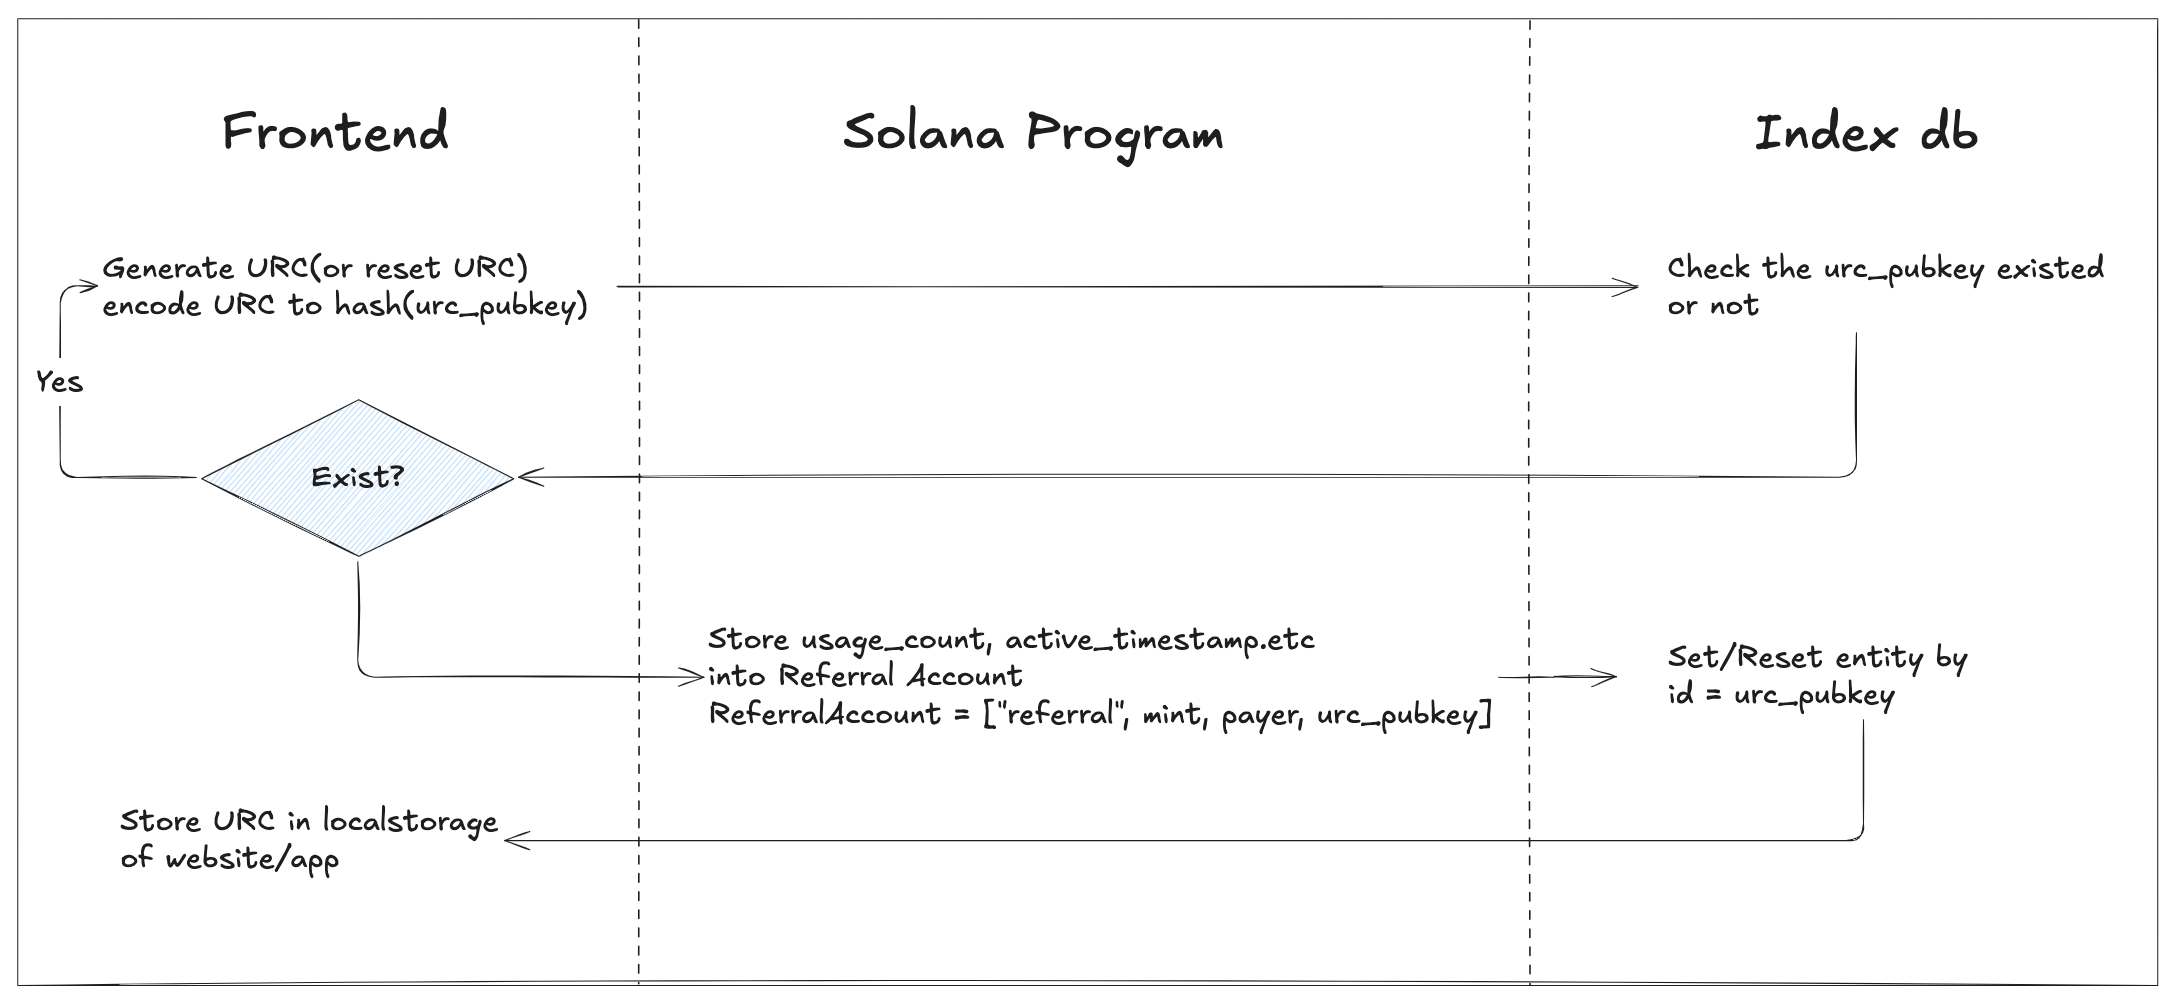
\includegraphics[width=400px]{urc_workflow}

\subsection{7 - 流动性}\label{ux6d41ux52a8ux6027}

铸造费用最终将注入去中心化交易所的流动性池,在其中可以赚取交易费用。

\subsubsection{7.1 -
流动性池的代币}\label{ux6d41ux52a8ux6027ux6c60ux7684ux4ee3ux5e01}

总代币供应量的一部分将分配给流动性池,作为SOL/代币对。这部分分配在铸造期间进入专用流动性账户。一旦满足某些条件(例如,第一个时代完成),这些代币连同交易费用(SOL)将自动添加到流动性池中。

\begin{itemize}
\tightlist
\item
  \(M_a\):每次铸造的代币数量(见3.1.4,3.1.4)
\item
  \(r_l\):初始流动性池相对于总发行量的比例,\(r_l < 1\)
\item
  \(L\):每次铸造事件进入流动性专用账户的代币数量
\end{itemize}

\begin{equation}
L = \frac{M_a \cdot r_l}{1 - r_l}
\end{equation}

因为代币总供应量为: \begin{equation}
TotalSupply = \sum_{i=1}^{E}(C \cdot T_0 \cdot \frac{1-f^{E}}{1-f})=C \cdot T_0 \cdot \frac{1-f^{E}}{1-f}
\end{equation}

初始化流动性池的代币为:

\begin{equation}
InitLiquidity = TotalSupply * \frac{r_l}{1-r_l} = C \cdot T_0 \cdot r_l \cdot \frac{1-f^{E}}{(1-f) \cdot (1-r_l)}
\end{equation}

\subsubsection{7.2 - 铸造费用}\label{ux94f8ux9020ux8d39ux7528}

铸造费用在6.2.2节中描述。铸造费用的分配如下:

\begin{itemize}
\tightlist
\item
  URC提供者:0-5\%
\item
  协议费用:5\%
\item
  流动性池:90-95\%
\end{itemize}

\subsubsection{7.3 -
初始化流动性池时的预计价格}\label{ux521dux59cbux5316ux6d41ux52a8ux6027ux6c60ux65f6ux7684ux9884ux8ba1ux4ef7ux683c}

根据去中心化交易所的\textbf{AMM},初始化流动性池时的代币价格为:

\begin{equation}
Price = \frac{0.90 \cdot TotalFee}{InitLiquidity}
\end{equation}

由于总铸造费用是一个范围: \begin{equation}
TotalFee \in [\frac{P_0 \cdot T_0}{M_0} \cdot C_e, \frac{P_0 \cdot T_0}{M_0} \cdot 101 \cdot (1.01^{C_e}-1)]
\end{equation}

因此,初始化流动性池时的最低价格为: \begin{equation}
P_{low} = \frac{P_0 \cdot C_e \cdot (1-r_l)(1-f)}{M_0 \cdot C \cdot r_l \cdot (1-f^E)}*0.90
\end{equation}

最高价格为: \begin{equation}
P_{high} = \frac{101 \cdot P_0 \cdot (1.01^{C_e}-1)(1-r_l)(1-f)}{M_0 \cdot C \cdot r_l \cdot (1-f^E)}*0.90=\frac{101 \cdot (1.01^{C_e}-1)}{C_e} \cdot P_{low}
\end{equation}

在上述公式中,\(C_e = E \cdot C\)(\(C\)是每个时代的周期数,\(E\)是时代数)

\subsection{8 退款}\label{ux9000ux6b3e}

铸造证明(PoM)是一种根据时间动态调整铸造规模的新代币发行模式。其核心逻辑如下:

\begin{itemize}
\tightlist
\item
  \textbf{动态成本调整}:

  \begin{itemize}
  \tightlist
  \item
    当实际铸造时间\textbf{短于目标铸造时间}时,铸造规模减少,代币成本增加。
  \item
    当实际铸造时间\textbf{等于或长于目标铸造时间}时,铸造数量和代币成本保持不变。
  \end{itemize}
\item
  \textbf{激励机制}:

  \begin{itemize}
  \tightlist
  \item
    该机制通过成本增加激励早期参与者,推动铸造活动。
  \item
    然而,它也可能导致后期参与者的成本过高,影响公平性。
  \end{itemize}
\end{itemize}

\subsubsection{8.1
退款机制的介绍与设计}\label{ux9000ux6b3eux673aux5236ux7684ux4ecbux7ecdux4e0eux8bbeux8ba1}

为解决上述问题,PoM引入了\textbf{退款}作为辅助约束,以确保公平性和保护参与者。其关键点如下:

\paragraph{8.1.1
目标时代锁定:}\label{ux76eeux6807ux65f6ux4ee3ux9501ux5b9a}

在目标时代期间,所有筹集的铸造费用都被锁定在一个特殊的金库中,参与者可以随时发起退款。

\paragraph{8.1.2
代币数量验证:}\label{ux4ee3ux5e01ux6570ux91cfux9a8cux8bc1}

退款时,系统将验证用户钱包中的代币总量是否等于铸造时的数量。

如果用户已转移或交易了部分代币,除非在钱包中补充相应数量的代币,否则退款将失败。

\paragraph{8.1.3
费用扣除规则:}\label{ux8d39ux7528ux6263ux9664ux89c4ux5219}

退款时,将扣除部分货币(例如,ETH/SOL)作为退款费用,以防止滥用。

如果铸造时使用了URC并获得了折扣,则在退款时将扣除已支付给URC提供者的奖励。

\paragraph{8.1.4
退款的优点与效果}\label{ux9000ux6b3eux7684ux4f18ux70b9ux4e0eux6548ux679c}

\begin{itemize}
\tightlist
\item
  \textbf{公平性保障}:

  \begin{itemize}
  \tightlist
  \item
    通过退款,后期参与者无需承担过高的铸造成本,确保公平参与。
  \item
    铸造费用的动态调整与退款机制共同作用,避免因``热铸造''导致的成本激增。
  \end{itemize}
\item
  \textbf{防止女巫攻击}:

  \begin{itemize}
  \tightlist
  \item
    由于后期参与者可能发起退款,女巫攻击者在早期干预的动机被削弱。
  \item
    该机制通过经济激励和约束有效降低恶意行为的概率。
  \end{itemize}
\item
  \textbf{社区模拟验证}:

  \begin{itemize}
  \tightlist
  \item
    社区内进行的模拟测试显示,退款显著提高了铸造过程的公平性和参与者满意度。
  \item
    最直接的结果是,由于退款风险,女巫攻击者减少了恶意活动,进一步优化了生态系统的健康。
  \end{itemize}
\end{itemize}

\subsubsection{8.2
退款并非随时可用}\label{ux9000ux6b3eux5e76ux975eux968fux65f6ux53efux7528}

请注意,退款仅在目标时代期间可用。目标时代结束后,铸造费用将用于初始化流动性池,退款功能将被禁用。

\subsection{9 -
完整案例研究}\label{ux5b8cux6574ux6848ux4f8bux7814ux7a76}

以下是在\textbf{Solana}区块链上部署铸造证明(PoM)机制的综合案例研究。

\subsubsection{9.1 - 参数}\label{ux53c2ux6570}

\begin{itemize}
\tightlist
\item
  总供应量:1,000,000,000代币
\item
  第一个时代每次铸造的目标规模(\(M_0\)):10,000代币
\item
  第一个时代每个周期的目标铸造规模(\(T_0\)):1,000,000代币
\item
  每个周期的最小铸造实例数:100
\item
  目标时代(\(E\)):1,第一个时代完成后,持有者可以转移代币,流动性池初始化。
\item
  每个时代的周期数(\(C\)):250
\item
  目标铸造天数:30天
\item
  减少因子(\(f\)):0.75
\item
  流动性代币百分比(\(r_l\)):10\%
\item
  每次铸造的费用(\(P_0\)):2美元每次铸造(0.0002美元/代币)
\item
  每个周期的目标铸造时间:173分钟(约3小时)
\item
  初始化流动性池时生成的LP代币处理方式:\textbf{全部销毁}
\item
  达到目标时代\#1时:

  \begin{itemize}
  \tightlist
  \item
    总供应量:250,000,000代币(最大供应量的25\%)
  \item
    总周期数:250
  \item
    铸造次数:\textgreater= 25,000
  \item
    总铸造费用:50,200美元至223,050美元
  \item
    初始化流动性池时的价格:0.001807美元至0.008030美元
  \end{itemize}
\end{itemize}

\subsubsection{9.2 -
铸造流程(技术上)}\label{ux94f8ux9020ux6d41ux7a0bux6280ux672fux4e0a}

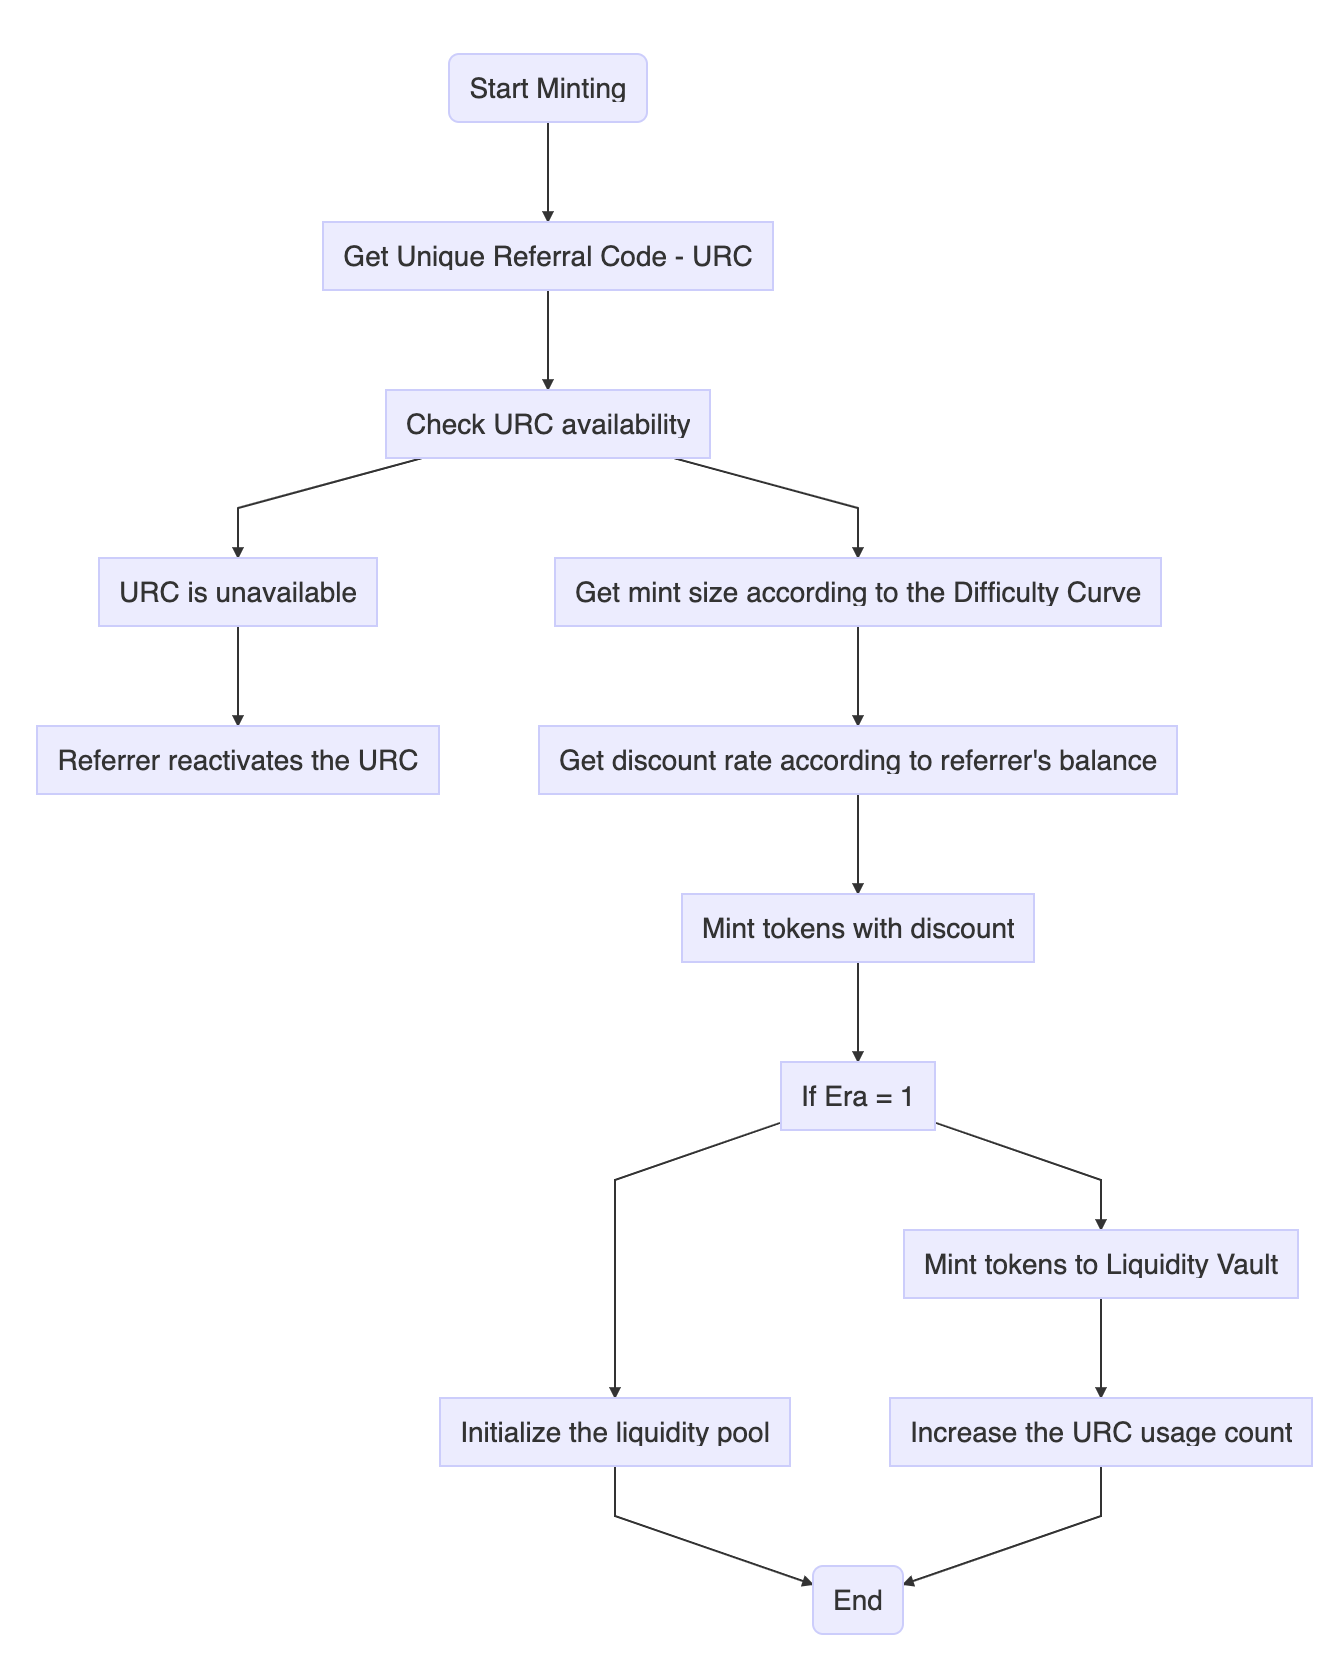
\includegraphics[width=400px]{mint_workflow}

\subsubsection{9.3 -
初始化流动性池流程(技术上)}\label{ux521dux59cbux5316ux6d41ux52a8ux6027ux6c60ux6d41ux7a0bux6280ux672fux4e0a}

任何人都可以初始化流动性,唯一条件是时代 \textgreater{} 1。

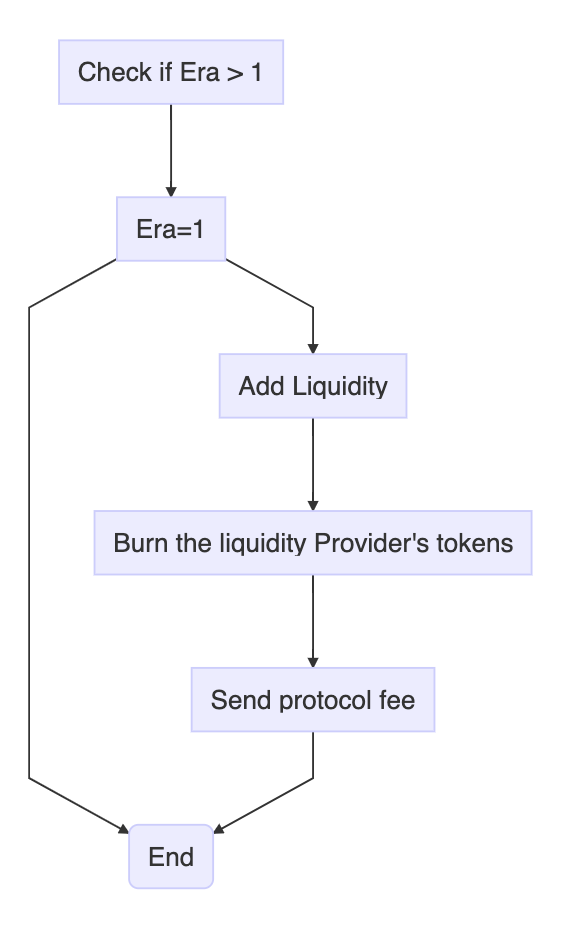
\includegraphics[width=200px]{initialize_liquidity_workflow}

\end{document}
